\documentclass[compress]{beamer}

\usepackage[utf8]{inputenc}
\usepackage{amsmath}
\usepackage{graphicx}
\usepackage{xcolor}
\usepackage[autostyle]{csquotes}
\usepackage{tikz,pgfplots}
\pgfplotsset{compat=newest}
\pgfplotsset{plot coordinates/math parser=false}
\usepackage{booktabs}
\usepackage[normalem]{ulem}
\usepackage{enumitem}
\usepackage{hyperref}

\usepackage[backend=bibtex,style=authoryear,citestyle=authoryear]{biblatex}
\addbibresource{SCOPF_literature.bib}


\setlist[description]{leftmargin=0pt}
\setitemize{label=\usebeamerfont*{itemize item}%
  \usebeamercolor[fg]{itemize item}
  \usebeamertemplate{itemize item}}

% Beamer Settings
\usetheme{Frankfurt}
\setbeamertemplate{items}[circle]
\setbeamertemplate{enumerate items}[default]
\setbeamertemplate{blocks}[rounded][shadow=false]
\setbeamertemplate{navigation symbols}{}
\setbeamercovered{transparent}
\setbeamertemplate{bibliography item}[triangle]
\useoutertheme[subsection=false]{miniframes}
\makeatletter
\let\beamer@writeslidentry@miniframeson=\beamer@writeslidentry
\def\beamer@writeslidentry@miniframesoff{%
  \expandafter\beamer@ifempty\expandafter{\beamer@framestartpage}{}% does not happen normally
  {%else
    % removed \addtocontents commands
    \clearpage\beamer@notesactions%
  }
}
\newcommand*{\miniframeson}{\let\beamer@writeslidentry=\beamer@writeslidentry@miniframeson}
\newcommand*{\miniframesoff}{\let\beamer@writeslidentry=\beamer@writeslidentry@miniframesoff}
\makeatother


% Bibliography tuning
\AtEveryBibitem{
   \clearfield{month}
   \clearfield{series}
   \clearfield{venue}
   \clearname{editor}
   \clearlist{publisher}
   \clearlist{location} % alias to field 'address'
   \clearfield{doi}
   \clearfield{url}
   \clearfield{urlday}
   \clearfield{urlmonth}
   \clearfield{urlyear}
   \clearfield{venue}
   \clearfield{issn}
   \clearfield{isbn}
   \clearfield{urldate}
   \clearfield{eventdate}
   %\clearfield{pages}
   %\clearfield{booktitle}
   %\clearfield{journaltitle}
   %\clearfield{number}
   %\clearfield{volume}
}

\newcommand*{\emphc}[1]{\textbf{\underline{#1}}}
\newcommand*{\citec}[1]{(From \cite{#1})}
\newcommand*{\field}[1]{\mathbb{#1}}
\newcommand*{\R}{\field{R}} % real R
\DeclareMathOperator*{\argmax}{arg\,max}

\newcommand\norm[1]{\left\lVert#1\right\rVert}
% \newlength\fheight 
% \newlength\fwidth 
% \setlength\fheight{0.4\textheight} 
% \setlength\fwidth{0.4\textwidth}

\usepackage{remreset}% tiny package containing just the \@removefromreset command, to view circles for slides in Frankfurt theme
\makeatletter
\@removefromreset{subsection}{section}
\makeatother
\setcounter{subsection}{1}

\AtBeginSection[]
{
   \begin{frame}
        \frametitle{Agenda}
        \tableofcontents[currentsection]
   \end{frame}
}

\title{Security-constrained optimal power flows\\Advanced power system analysis}
\author{Camille Hamon\\camille.hamon@ntnu.no}
\date{11 October 2016}

% \AtBeginSection[] % Do nothing for \subsection*
% {
% \begin{frame}<beamer>
% \frametitle{Outline}
% \tableofcontents[currentsection,subsectionstyle=hide]
% \end{frame}
% }

\begin{document}
% Remove spacing around align environment
\setlength{\abovedisplayskip}{0pt}
\setlength{\belowdisplayskip}{0pt}
\setlength{\abovedisplayshortskip}{0pt}
\setlength{\belowdisplayshortskip}{0pt}
\nocite{*}
\miniframesoff
\begin{frame}[plain]
  \titlepage
\end{frame}
\miniframeson

\section{Introduction}

\begin{frame}
  \frametitle{Perspectives}
\blockquote[\cite{Cain2012History}]{Today, 50 years after the problem was formulated, we still do not have a fast, robust solution technique for the full ACOPF.  Finding a good solution technique for the full ACOPF could potentially save tens of billions of dollars annually.}

\noindent\rule[0.5ex]{\linewidth}{1pt}

\blockquote[2016, Analytic Research Foundations for the Next-Generation Electric Grid]{Recommendation 1: The Department of Energy should develop and test a full ac optimal power flow
(ACOPF) model with an optimization algorithm using all nodes in the market area, taking advantage of
supercomputers and parallel processing and respecting all thermal and voltage constraints.} 

\end{frame}

\begin{frame}
  \frametitle{Example}
  \begin{columns}
    \begin{column}{0.7\textwidth}
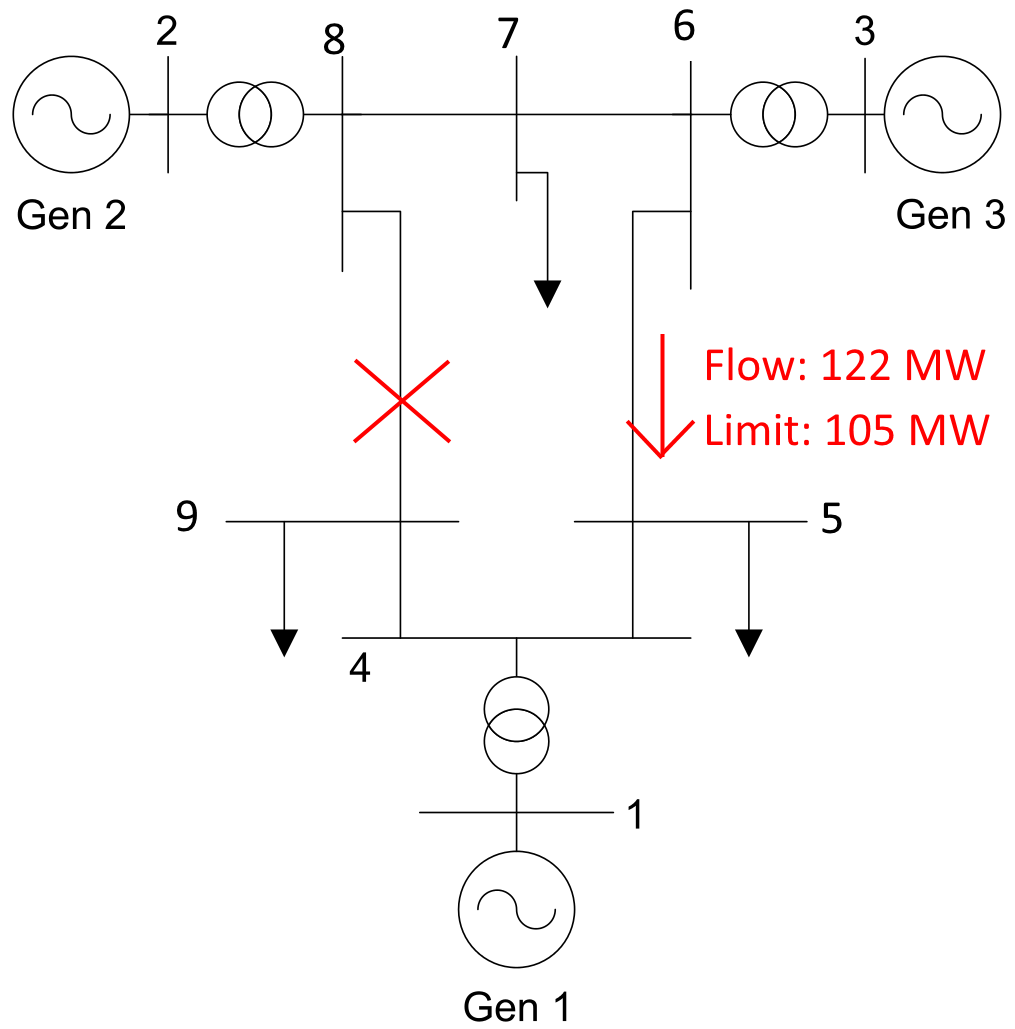
\includegraphics[width=\textwidth]{Figs/ieee9_fault_line_8-9.png}
    \end{column}
    \begin{column}{0.3\textwidth}
      What do you do?
    \end{column}
  \end{columns}
\end{frame}

\begin{frame}
  \frametitle{Example 2}
  \begin{columns}
    \begin{column}{0.6\textwidth}
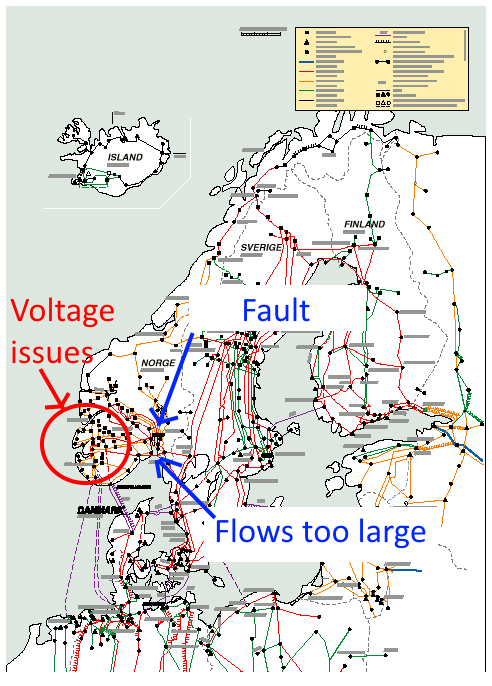
\includegraphics[width=\textwidth]{Figs/NordicPS_fault.png}
    \end{column}
    \begin{column}{0.3\textwidth}
      What do you do?
    \end{column}
  \end{columns}
\end{frame}

\begin{frame}{SCOPF - General formulation}
Security-constrained optimal power flows are \emphc{optimization problems} of the following form:
\vskip0.5cm
  \begin{align}
    \min & \quad \text{Cost of preventive and corrective actions} \\
    \text{subject to} & \quad \text{The system is secure}
  \end{align}
\vskip0.5cm
That is, we want to find \emphc{preventive} and \emphc{corrective} actions that make the system secure.
\end{frame}

\begin{frame}
\frametitle{Outline}  
Topics to discuss today:
\begin{itemize}
\item What is security?
\item When do transmission system operators need SCOPF?
\item What are preventive and corrective actions?
\item How to translate the power system problem ``ensuring security'' to mathematical equations that can be used in an optimisation framework?
\end{itemize}
\end{frame}

\section{Security}
\begin{frame}{What is security?}
\underline{Operational security} is defined for all European transmission system operators in \emph{ENTSO-E network code on operational security}:
\begin{block}{}
\textquote[From \cite{Entso-e2013Network}]{\textbf{Operational Security} means the Transmission System capability to retain a Normal State or to return to a Normal State as soon and as close as possible, and is characterized by thermal limits, voltage constraints, short-circuit current, frequency limits and stability limits} 
\end{block}
\end{frame}

\begin{frame}
  \frametitle{Dy Liacco's security diagram}
\centering  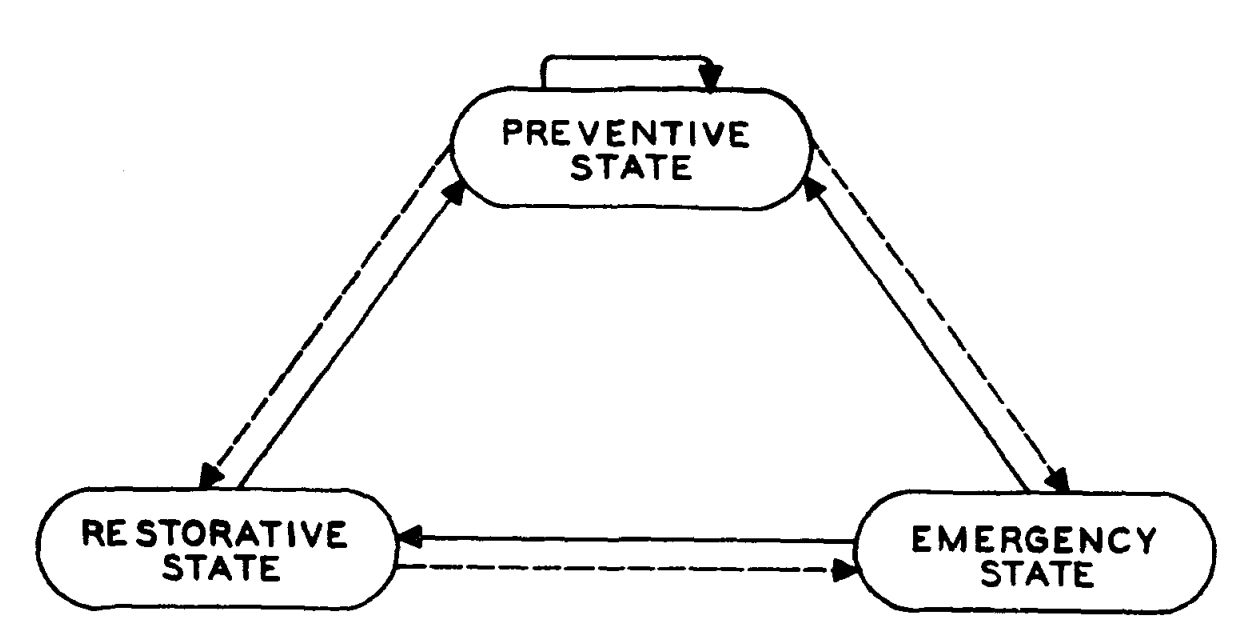
\includegraphics[width=0.8\textwidth]{Figs/DyLiacco_SecurityDiagram.png}\\
  \citec{DyLiacco1967Adaptive}
\end{frame}

\begin{frame}
  \frametitle{Dy Liacco's security diagram - State description}
\centering  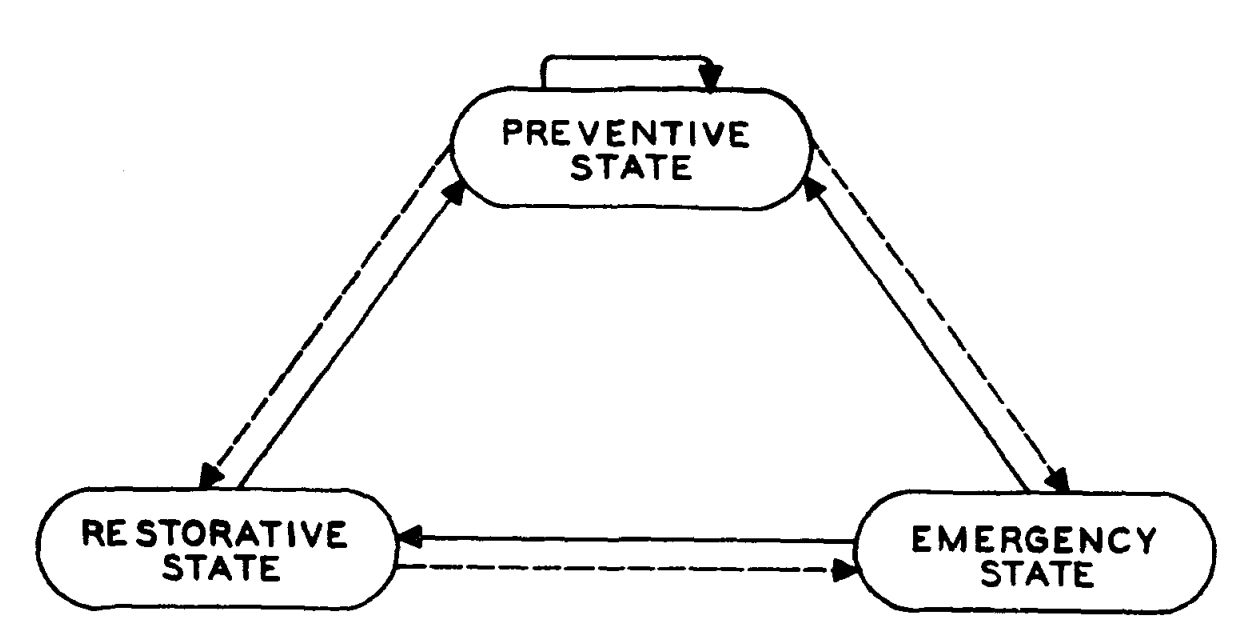
\includegraphics[width=0.4\textwidth]{Figs/DyLiacco_SecurityDiagram.png}
\begin{description}
  \item[Preventive (normal) state] All components within operating constraints\footnote{what are typical operating constraints?}. \underline{Preventive control actions}: anticipate threats (changes in load, RES production, outages of generators, lines, etc).
  \item[Emergency state] Stability lost or some operating constraints violated. \underline{Emergency control actions}: Stop the degradation of services.
  \item[Restorative state] Service outages (interruptions of supply for some customers) \underline{Restoration control actions}: Restore electricity supply to all customers.
  \end{description}
\end{frame}

\begin{frame}
\frametitle{Cihlar's security diagram}
\centering
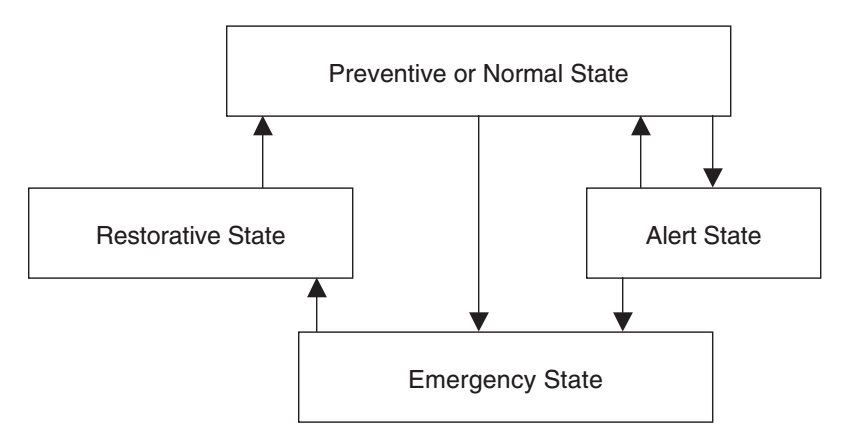
\includegraphics[width=0.6\textwidth]{Figs/Cihlar_SecurityDiagram.png}\\
\citec{Cihlar1969Electric}
\begin{description}
\item[Alert state] = Potential emergency. Operating constraints still satisfied (like in the normal state) but some operating constraints would be violated in case of a contingency (we would go to the emergency state should that contingency occur). \underline{Preventive control actions}: Actions to return to the normal state.
\end{description}
\end{frame}


\begin{frame}
\frametitle{Fink and Carlsen's security diagram}
\centering
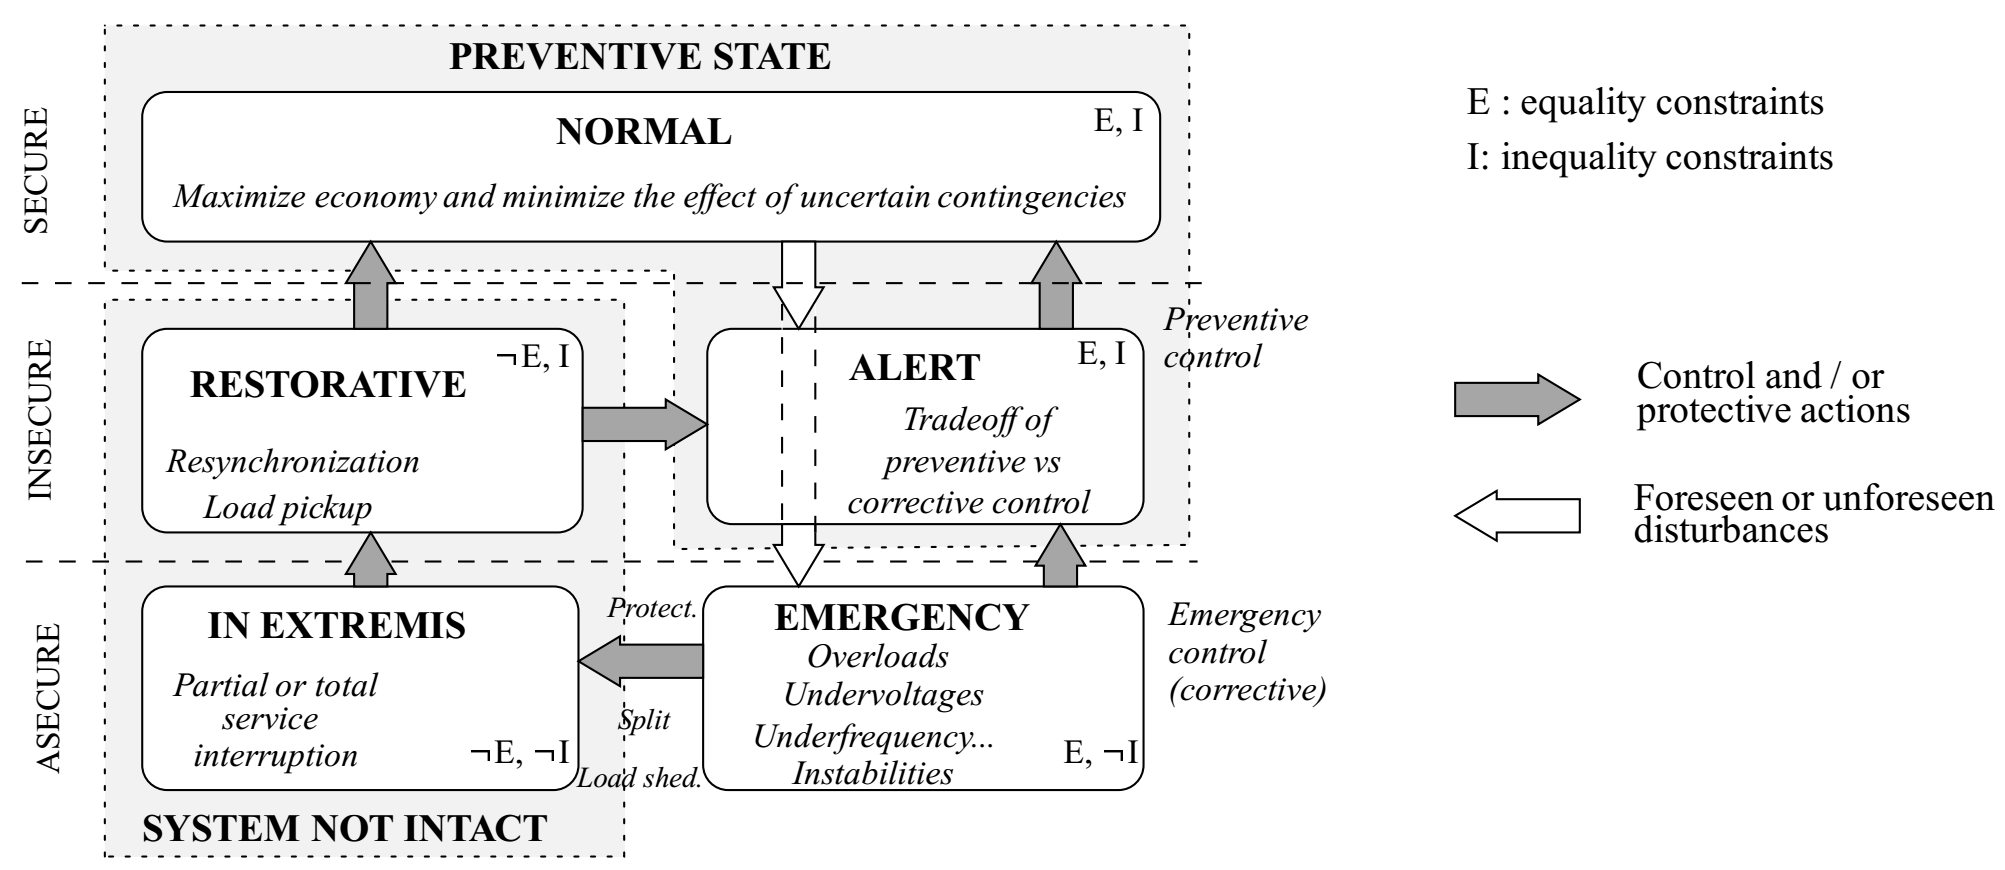
\includegraphics[width=\textwidth]{Figs/FinkCarlsen_SecurityDiagram.png}\\
\citec{Fink1978Operating}
\begin{description}
\item[In extremis state] Partial or total system collapse = Interruption of supply. \underline{Corrective actions}: Stop the collapse, and prevent the system from further degrading.
\end{description}
\end{frame}

\begin{frame}
  \frametitle{Today's security diagram}
  \begin{itemize}
  \item Fast forward almost 40 years to today: the same five states are still pivotal to the definition of security.
  \item See Article 8 in ENTSO-E network code on operational security (2013)
  \end{itemize}

\only<1>{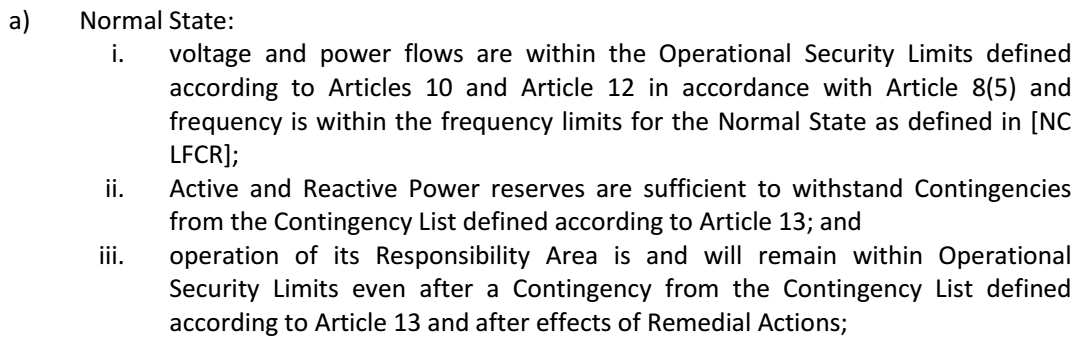
\includegraphics[width=0.9\textwidth]{Figs/NormalState.png}}
\only<2>{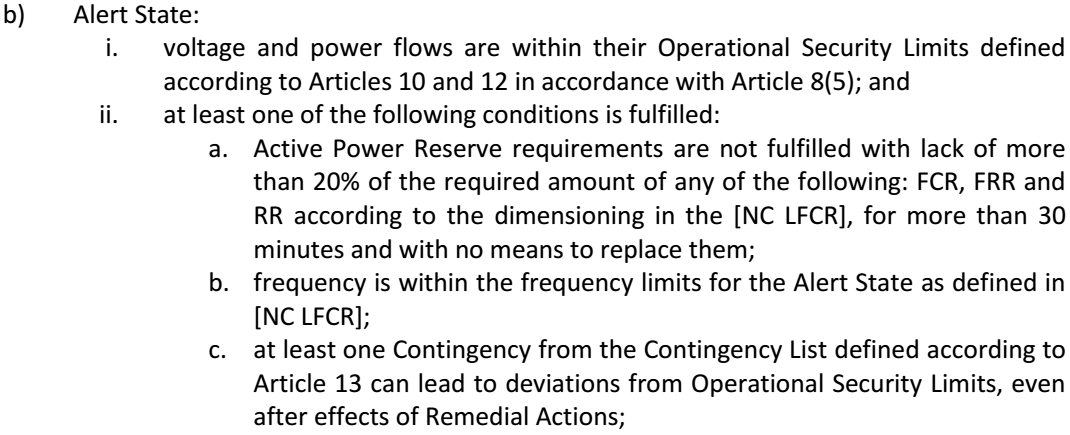
\includegraphics[width=0.9\textwidth]{Figs/AlertState.png}}
\only<3>{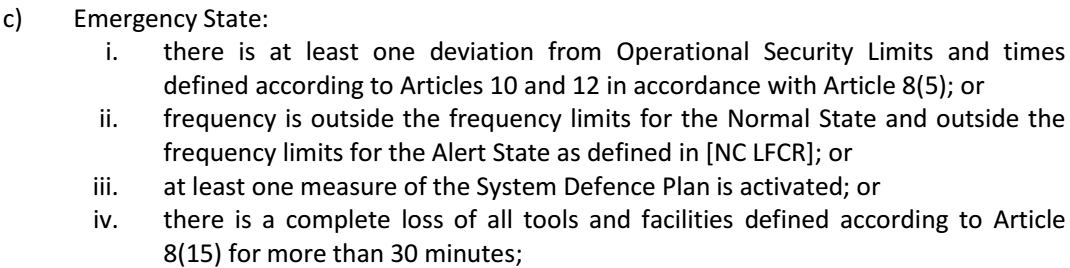
\includegraphics[width=0.9\textwidth]{Figs/EmergencyState.png}}
\only<4>{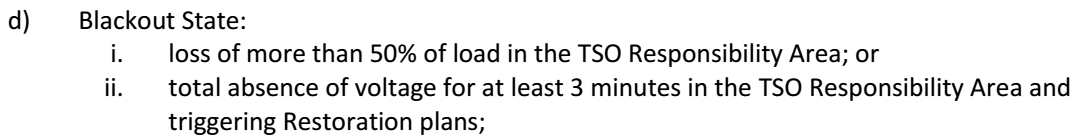
\includegraphics[width=0.9\textwidth]{Figs/BlackoutState.png}}
\only<5>{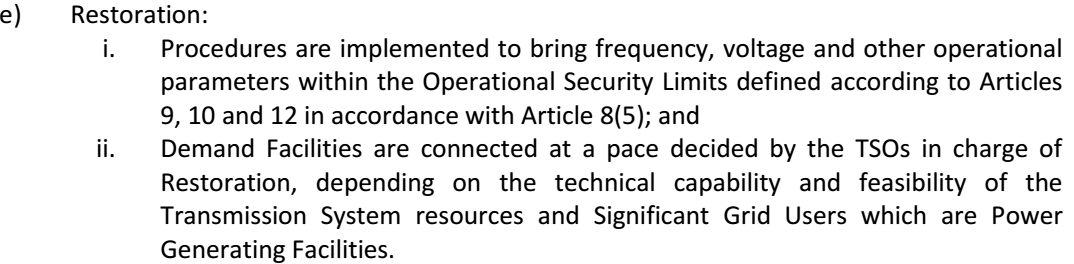
\includegraphics[width=0.9\textwidth]{Figs/RestorationState.png}}
\end{frame}

\begin{frame}
  \frametitle{Definition of security (Again)}
\underline{Operational security} is defined for all European transmission system operators by \emph{ENTSO-E network code on operational security}:
\begin{block}{}
\textquote[From \cite{Entso-e2013Network}]{\textbf{Operational Security} means the Transmission System capability to \underline{retain a Normal State} or to \underline{return to a Normal State} as soon and as close as possible, and is characterized by thermal limits, voltage constraints, short-circuit current, frequency limits and stability limits} 
\end{block}
\begin{block}{}
\textbf{Operational security limits} are cornerstones of the definition of security. Also called security constraints (``constraints'' is a mathematical term used in optimization).
\end{block}
\end{frame}

\begin{frame}
  \frametitle{Question 1}
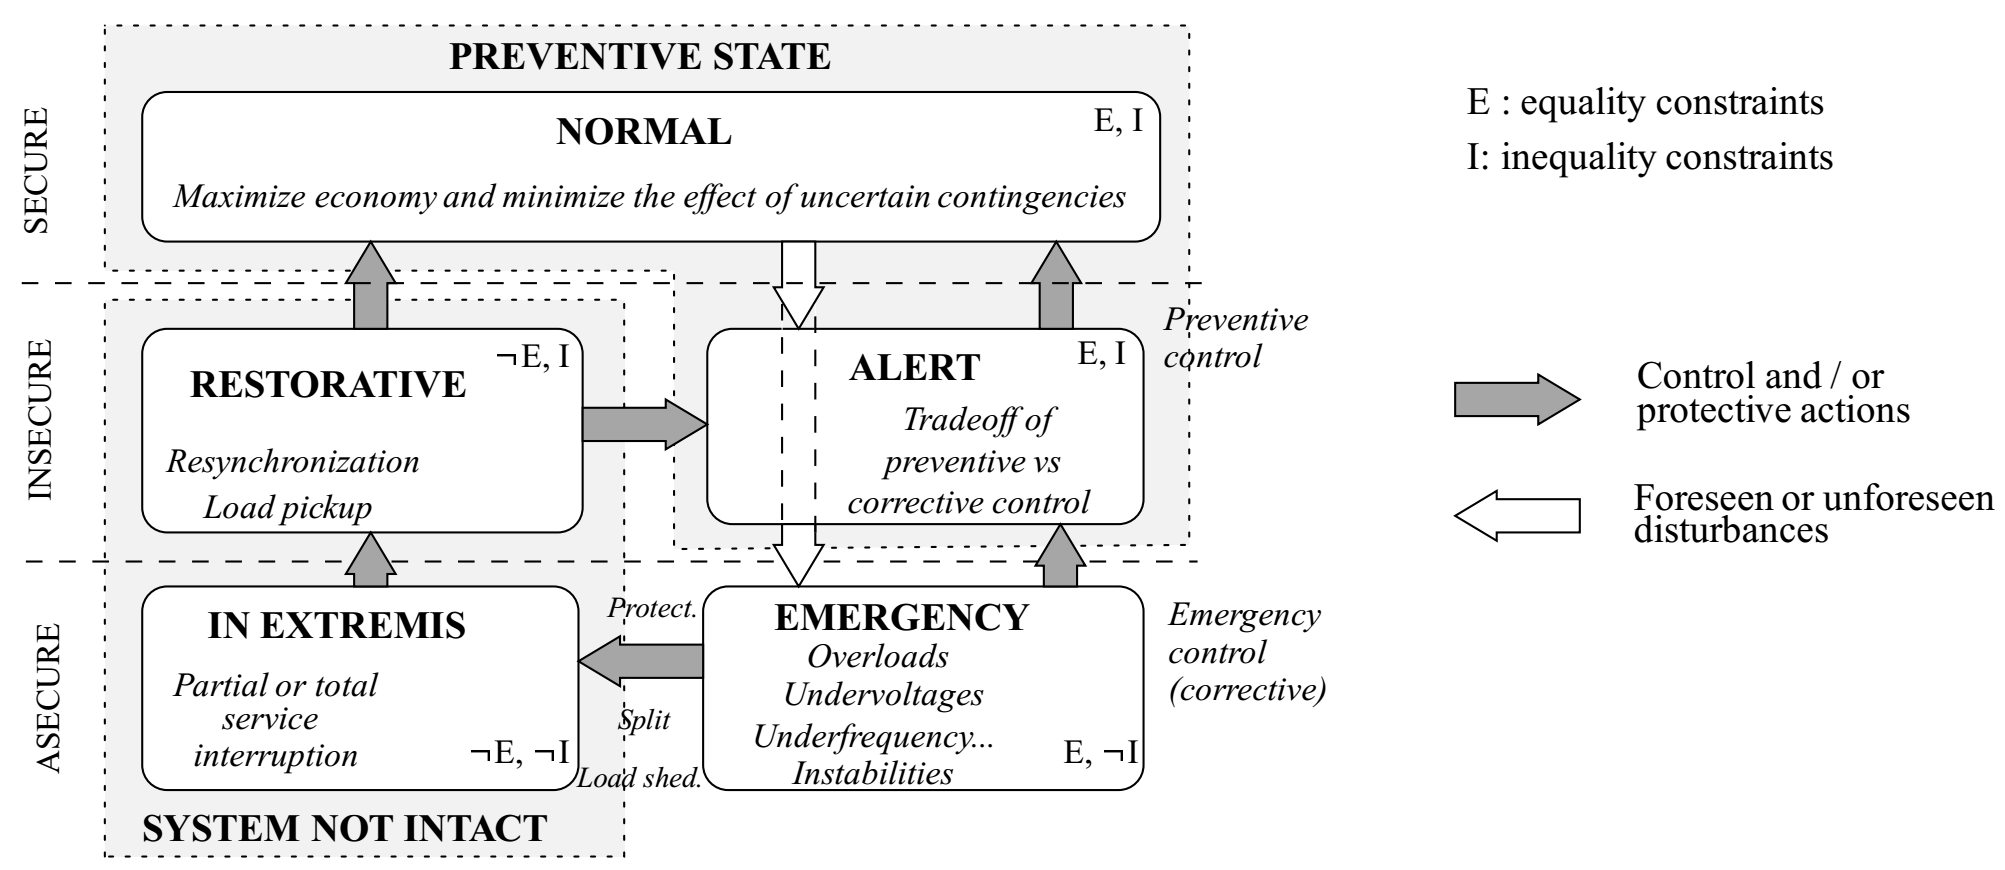
\includegraphics[width=\textwidth]{Figs/FinkCarlsen_SecurityDiagram.png}\\
\begin{itemize}
\item Suppose that no contingency has occurred. Contingency analyses show that the flow limits of one line would be exceeded if one specific contingency occured. In which state is the system?
\end{itemize}
\end{frame}


\begin{frame}
  \frametitle{Question 2}
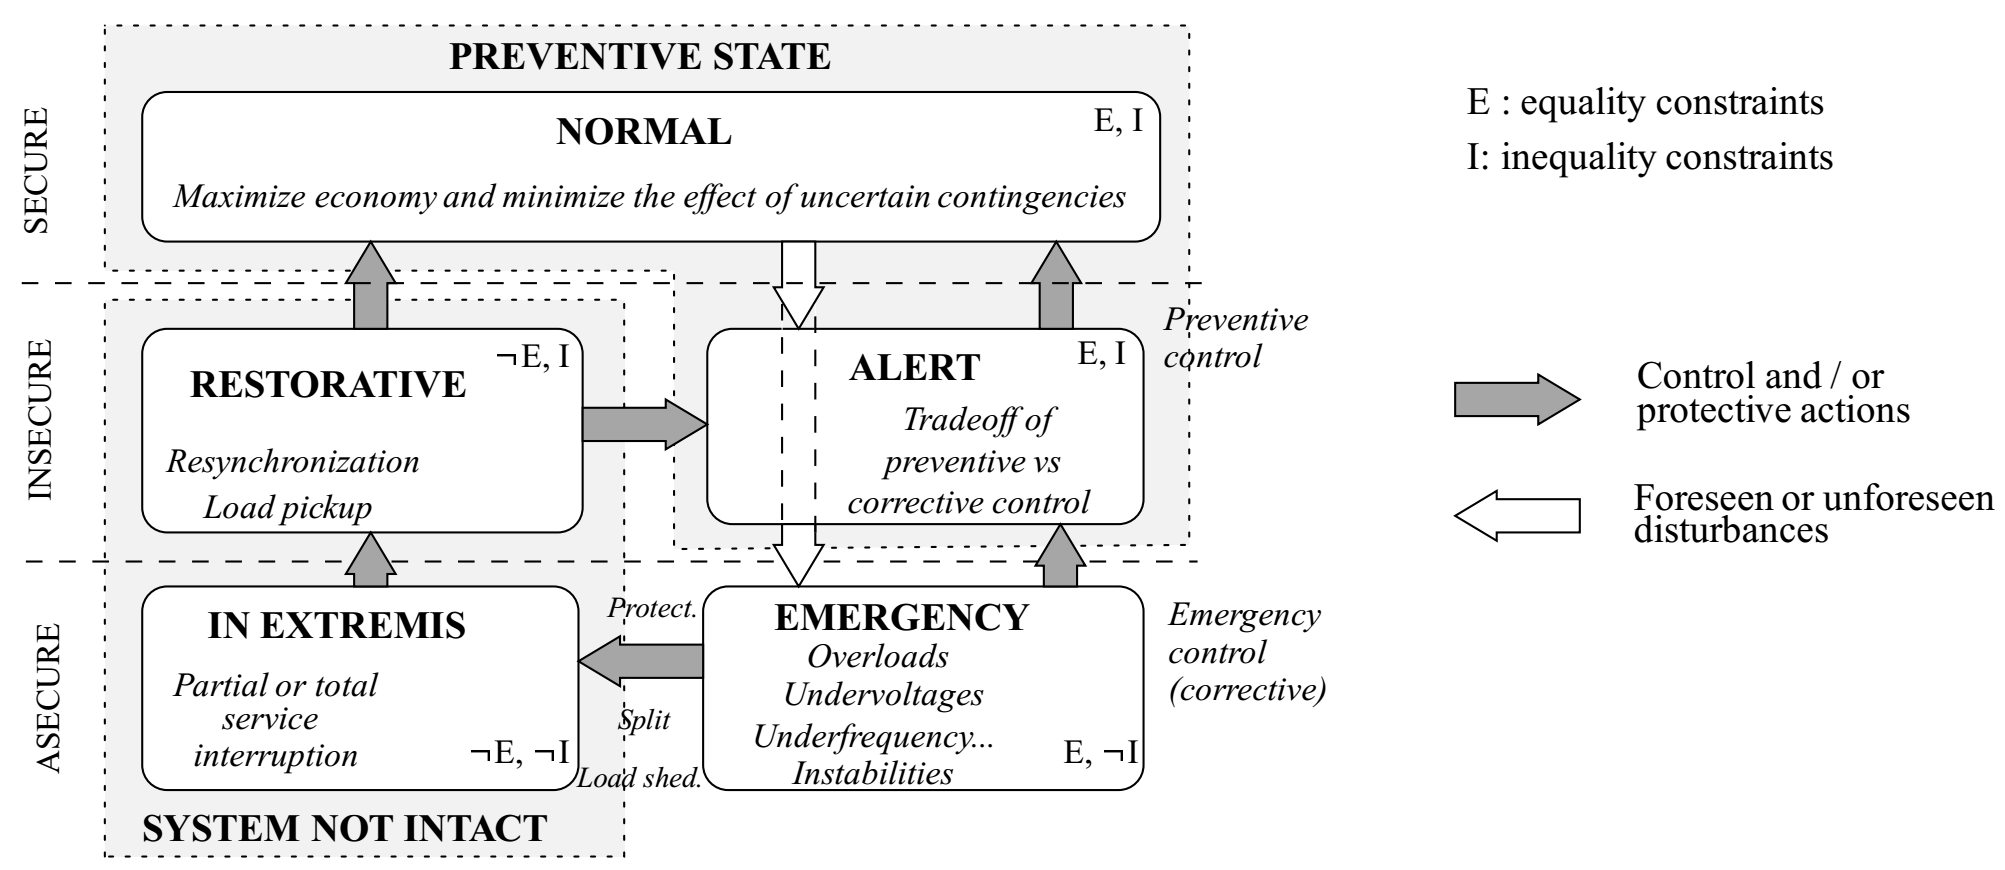
\includegraphics[width=\textwidth]{Figs/FinkCarlsen_SecurityDiagram.png}\\
\begin{itemize}
\item Suppose that a contingency has occurred and voltages in one area exceed their limits. In which state is the system?
\item Suppose further that no load shedding was necessary. In which state is the system?
\end{itemize}
\end{frame}

\begin{frame}
  \frametitle{Question 3}
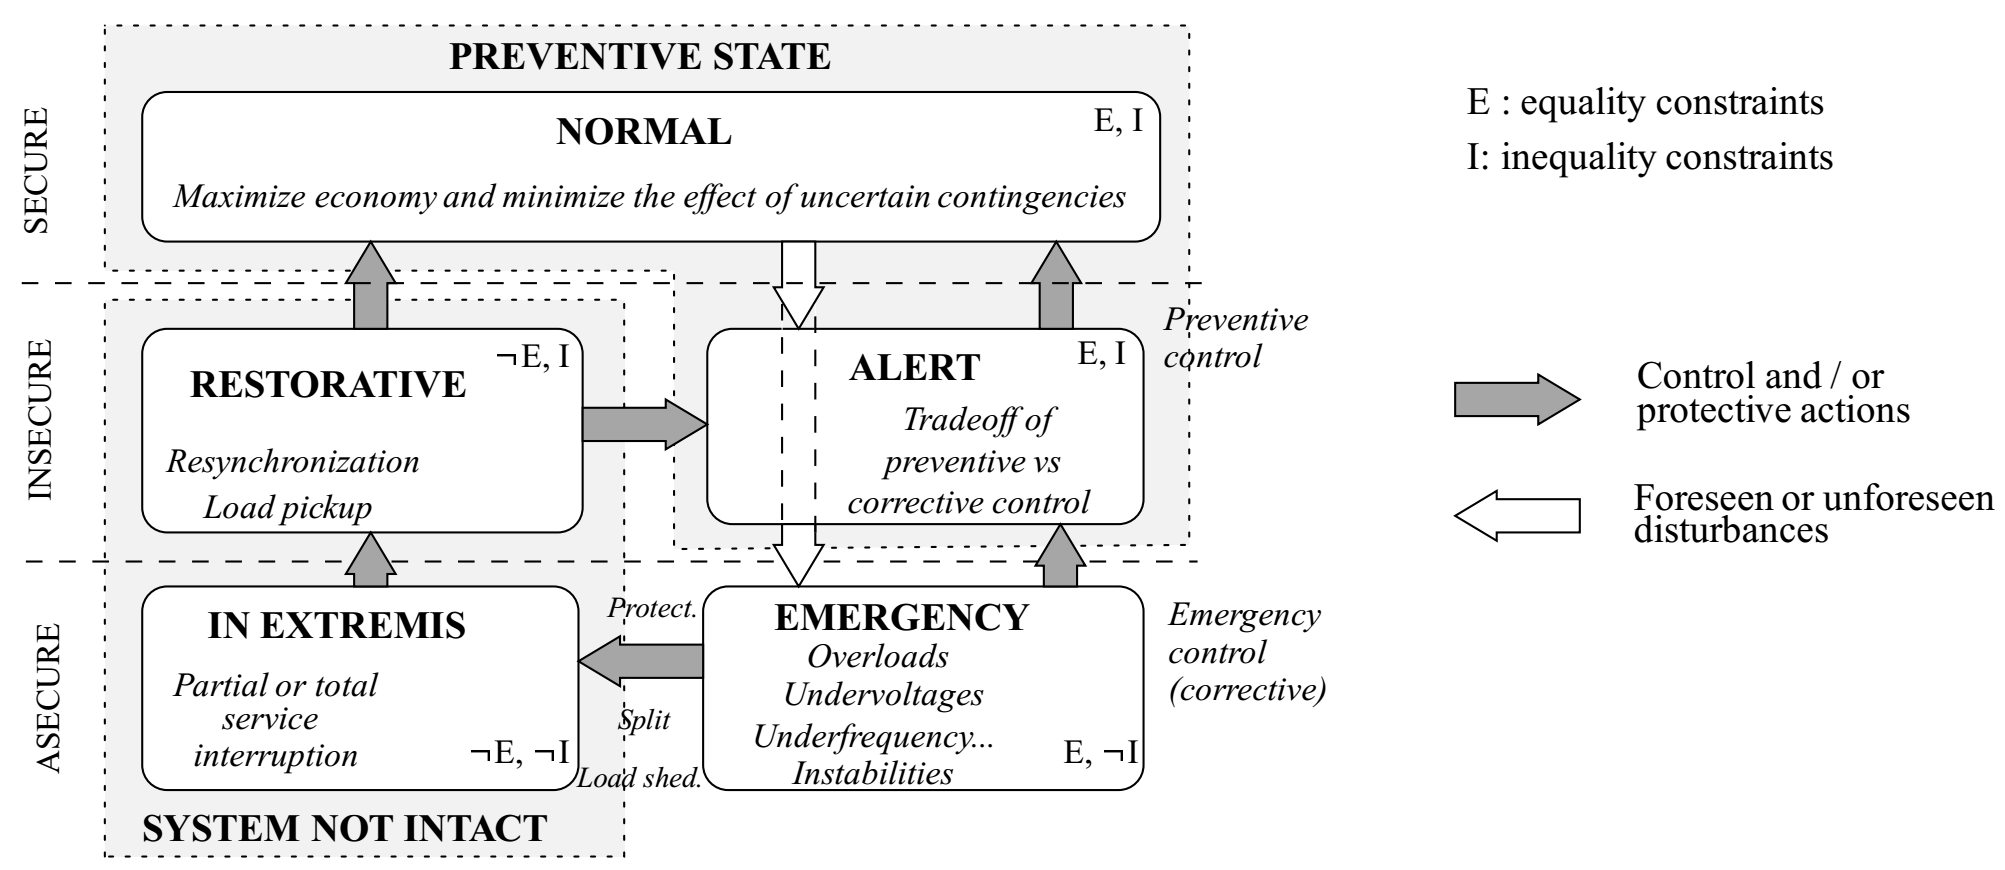
\includegraphics[width=\textwidth]{Figs/FinkCarlsen_SecurityDiagram.png}\\
\begin{itemize}
\item Suppose that a contingency has occurred and all limits are fulfilled. In which state is the system?
\end{itemize}
\end{frame}


\section{Security constraints}
\begin{frame}
\frametitle{Fink and Carlsen's security diagram}
\underline{Getting closer to a mathematical formulation:}
\centering
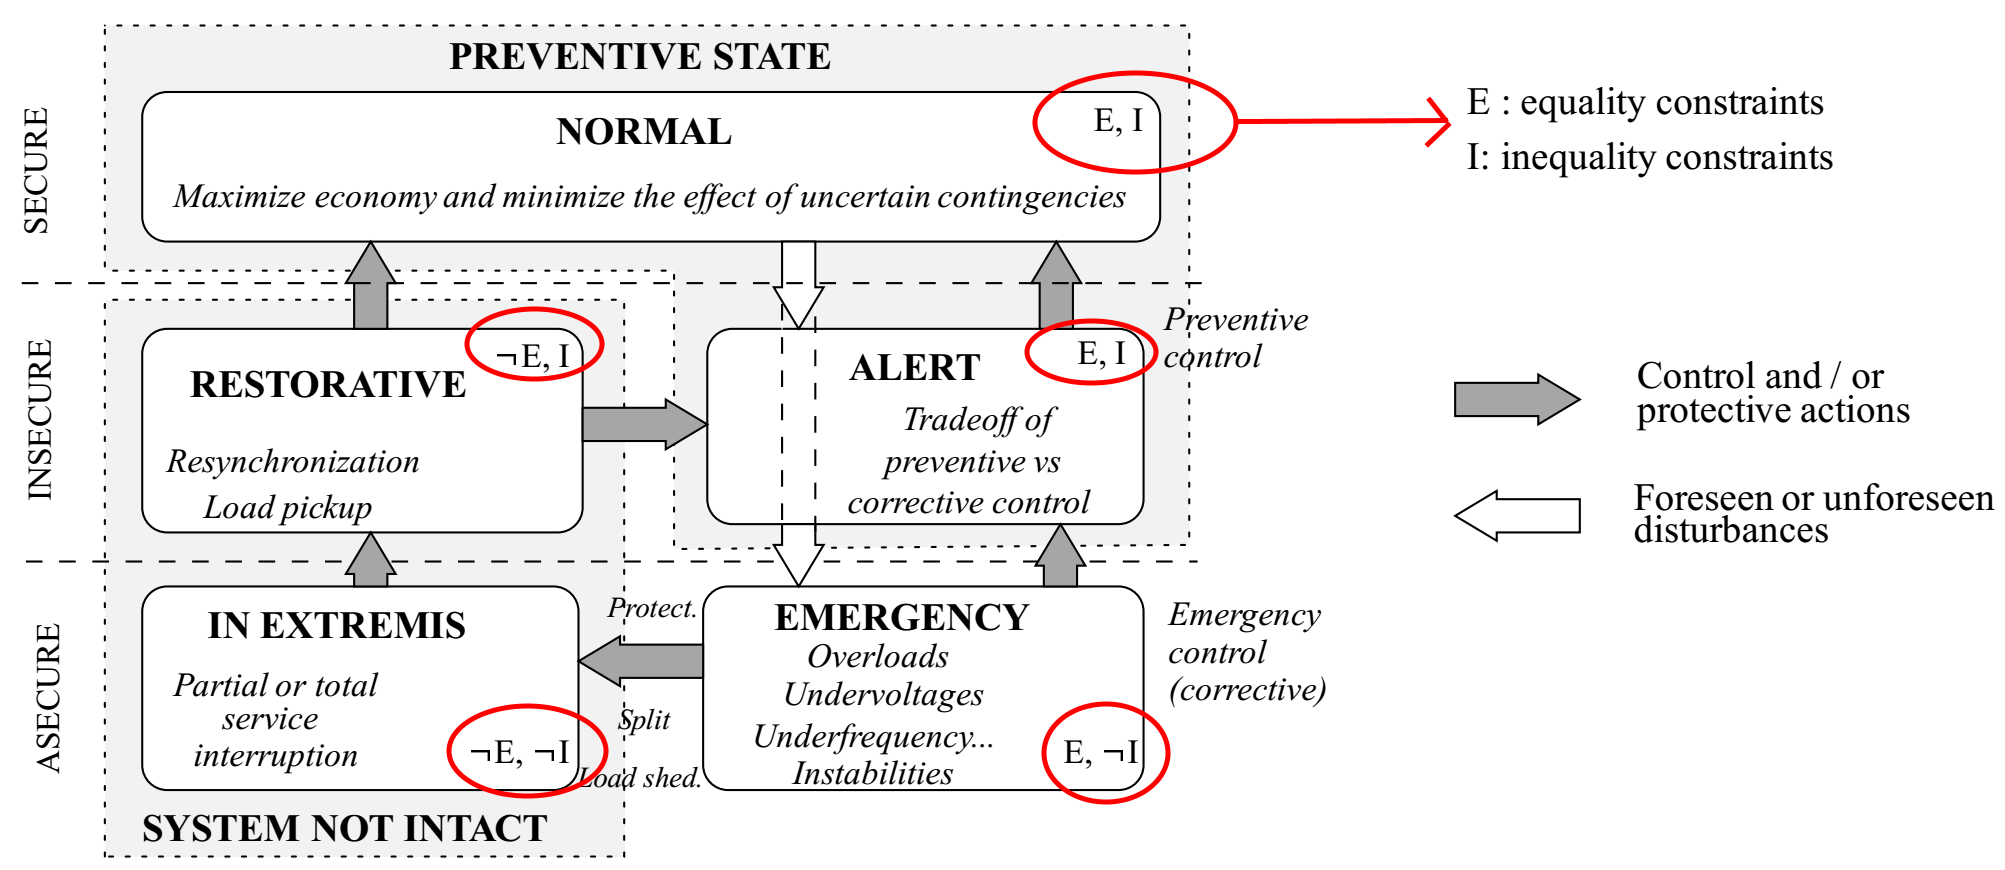
\includegraphics[width=\textwidth]{Figs/FinkCarlsen_SecurityDiagram_Highlight.png}\\
\citec{Fink1978Operating}
\begin{itemize}
\item What are equality and inequality constraints?
\end{itemize}
\end{frame}

\begin{frame}
\frametitle{Security constraints in SCOPF}
\begin{block}{}
\textquote[From \cite{Entso-e2013Network}]{\textbf{Operational Security} means the Transmission System capability to retain a Normal State or to return to a Normal State as soon and as close as possible, and is characterized by \underline{thermal limits}, \underline{voltage constraints}, short-circuit current, frequency limits and \underline{stability limits}} 
\end{block}

Typically:
\begin{itemize}
\item Short-circuit currents are dealt with by protection systems.
\item Frequency limits are dealt with by frequency control reserves.
\end{itemize}
Security constraints left:
\begin{itemize}
\item Thermal limits.
\item Voltage constraints.
\item Stability limits.
\end{itemize}  
\end{frame}

\begin{frame}
\frametitle{Thermal limits}
\begin{block}{Power system perspective}
Thermal limits (or thermal ratings) are limits on loading of components such as lines, cables and transformers.

Two types of limits:
\begin{itemize}
\item Long-term (or continuous) limits: components can operate a long time without problem if these limits are fulfilled.
\item Short-term limits (or emergency limits): These limits can be sustained by components \underline{only} for a short time (e.g. 15 minutes).
\end{itemize}
\end{block}
\begin{block}{Math formulation}
  \begin{align*}
    P_{l} \leq P_l^{\text{max}}, \; \forall \text{ lines } l.
  \end{align*}
\footnotesize \underline{Question for later:} How to distinguish long-term and short-term limits in the mathematical formulation?
\end{block}
\end{frame}

\begin{frame}
\frametitle{Example}
\begin{columns}
  \begin{column}{0.5\textwidth}
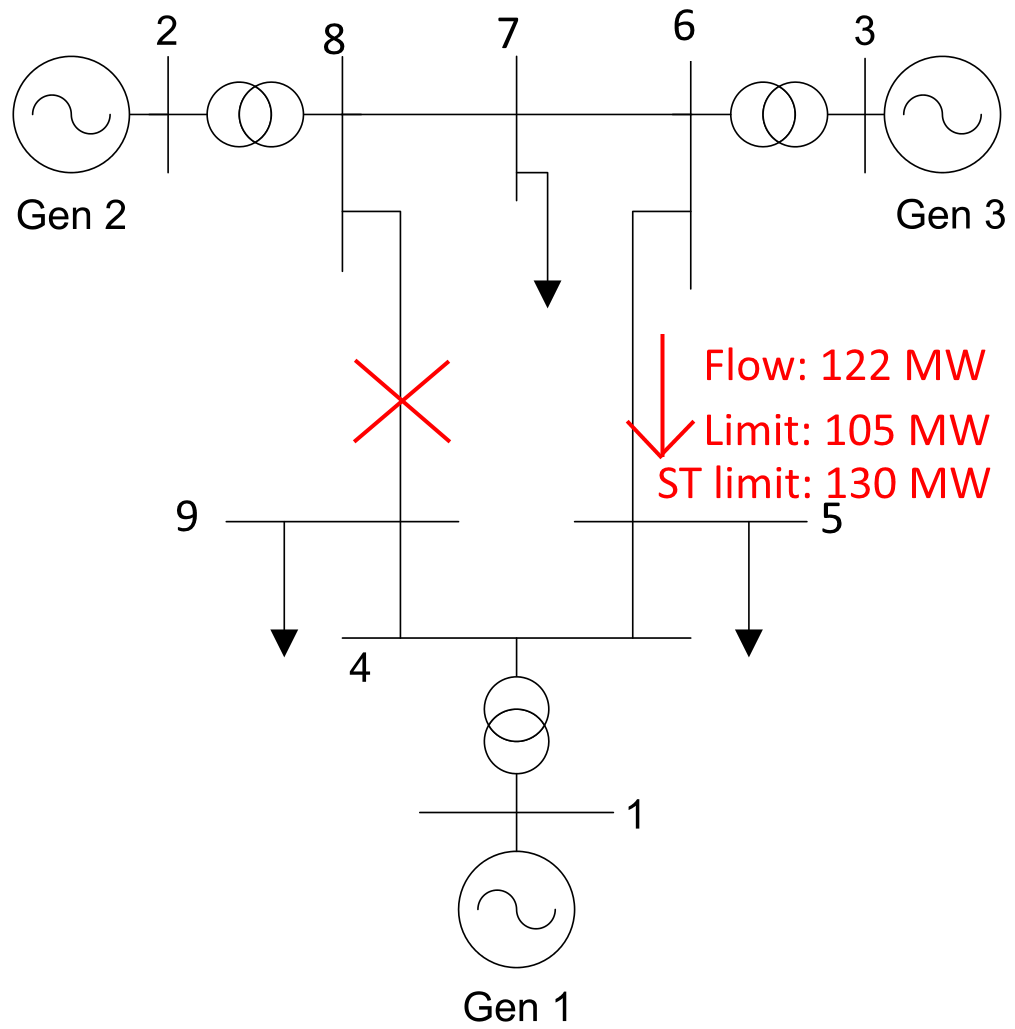
\includegraphics[width=\textwidth]{Figs/ieee9_fault_line_8-9_stratings.png}
  \end{column}
  \begin{column}{0.5\textwidth}
    \begin{itemize}
    \item The flow is acceptable for 15 minutes
    \item TSO would have to take actions within 15 minutes
    \end{itemize}
  \end{column}
\end{columns}
\end{frame}

\begin{frame}
  \frametitle{Voltage constraints}
  \begin{block}{Power system perspective}
From ENTSO-E network code on operational security:

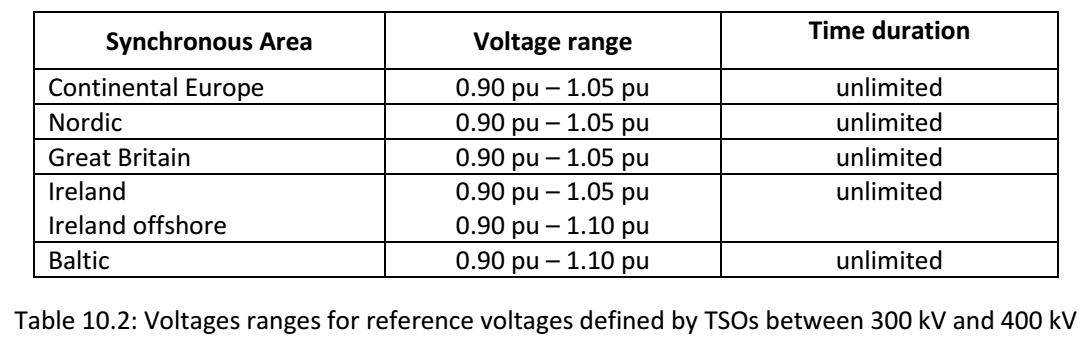
\includegraphics[width=0.9\textwidth]{Figs/ENTSOE-NCOS-VoltageRanges.png}    \end{block}
\begin{block}{Math formulation}
  \begin{align*}
  V_i^{\text{min}} \leq V_i \leq V_i^{\text{max}}, \; \forall \text{ buses } i.
  \end{align*}
\end{block}
\end{frame}

\begin{frame}
  \frametitle{Voltage constraints - 2}
\begin{columns}
\begin{column}{0.3\textwidth}
What happens if voltages exceed the range?\\
The answer is in \emph{ENTSO-E network code on Requirements for Grid Connection Applicable to all Generators (RfG) of 2016}:   
\end{column}
\begin{column}{0.7\textwidth}
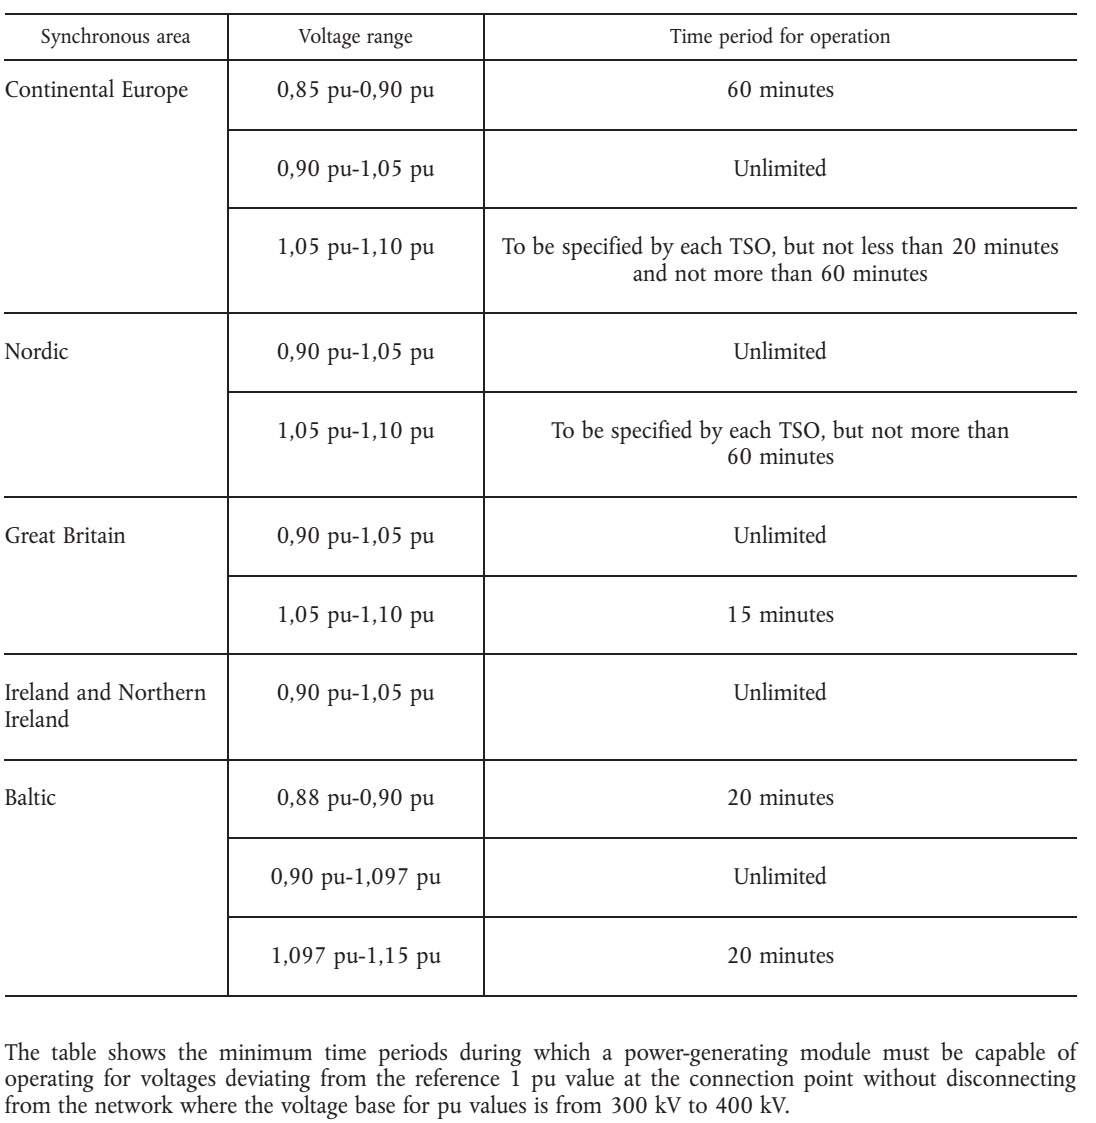
\includegraphics[width=1\textwidth]{Figs/ENTSOE-NCOS-EmergencyVoltageRanges.png}
\end{column}
\end{columns}
\end{frame}

\begin{frame}
  \frametitle{Example}
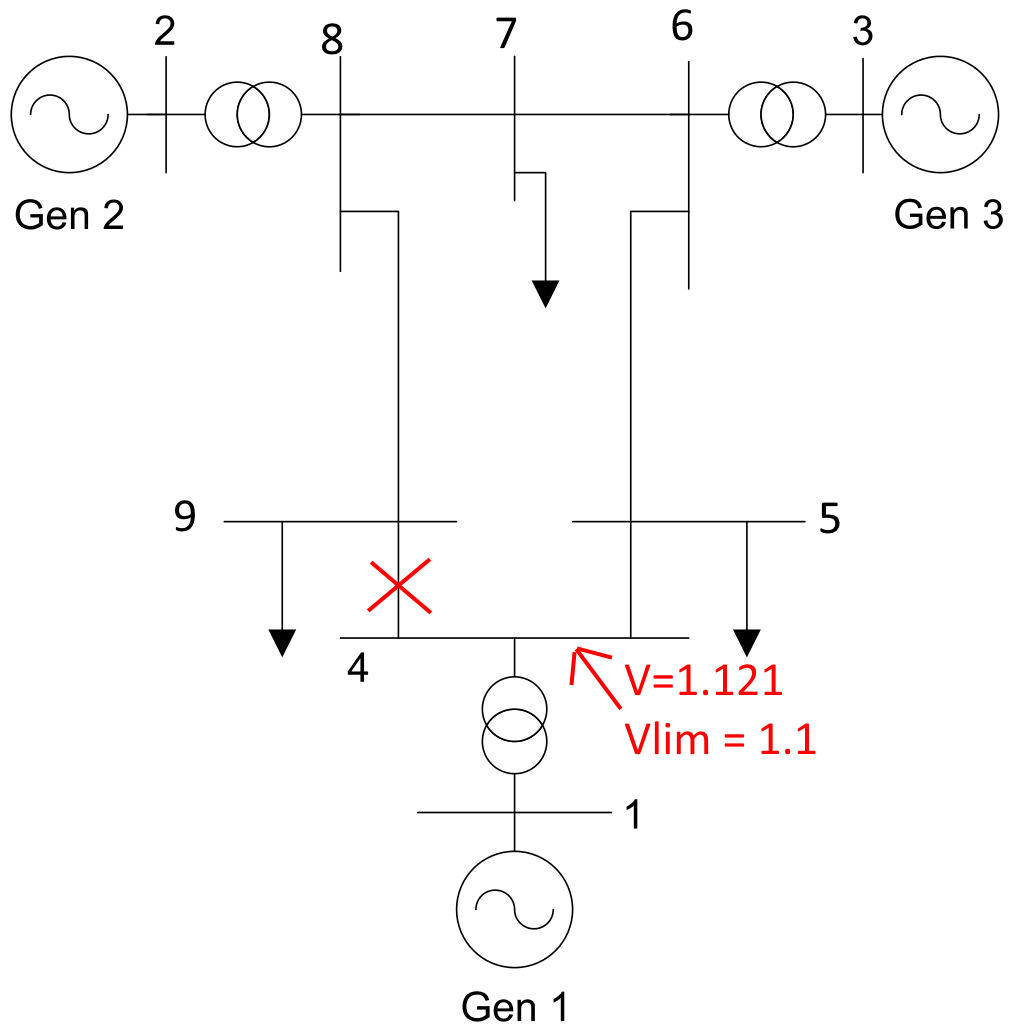
\includegraphics[width=0.7\textwidth]{Figs/ieee9_fault_line_4-9_voltages.png}
\end{frame}

\begin{frame}
\frametitle{Stability constraints}
\begin{block}{Power system perspective}
Typically, stability constraints take the form of active power limits on critical interfaces (=transmission corridors / lines). 

\begin{columns}
\begin{column}{0.45\textwidth}
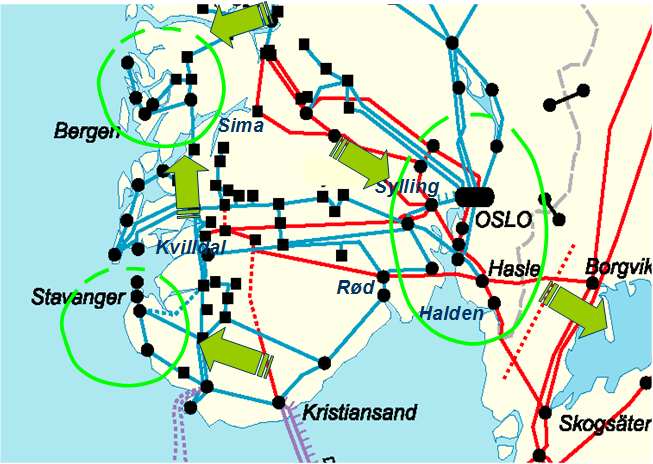
\includegraphics[width=1\textwidth]{Figs/Hasle.png}    
\end{column}
\begin{column}{0.45\textwidth}
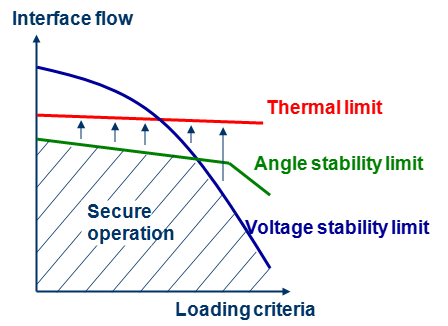
\includegraphics[width=1\textwidth]{Figs/SecurityLimits.png}
\end{column}
\end{columns}  
\end{block}
\begin{block}{Math formulation}
  \begin{align*}
    P_l \leq P_l^{\text{max}}, \; \forall \text{ critical interfaces } l.
  \end{align*}
\underline{Note:} \emph{same math formulation as thermal limits but fundamentally different constraints!}
\end{block}
\end{frame}

\begin{frame}
  \frametitle{Contingencies}
Remember:
\begin{block}{}
\textquote[From \cite{Entso-e2013Network}]{\textbf{Operational Security} means the Transmission System capability to \underline{retain a Normal State} or to \underline{return to a Normal State} as soon and as close as possible, and is characterized by thermal limits, voltage constraints, short-circuit current, frequency limits and stability limits} 
\end{block}
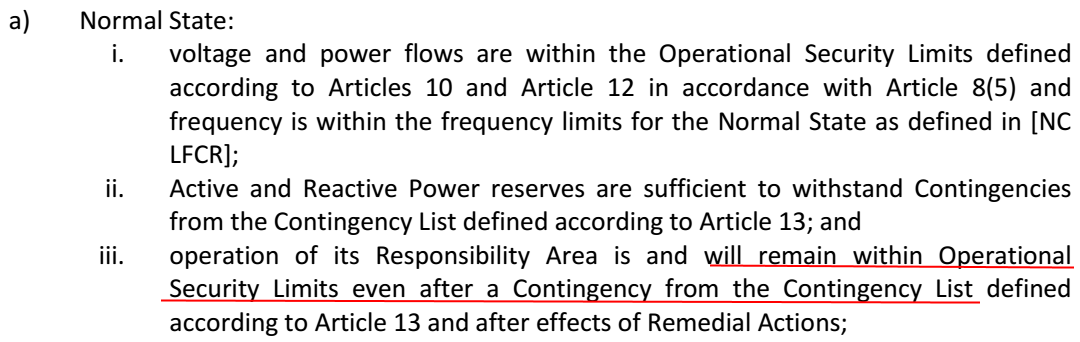
\includegraphics[width=0.9\textwidth]{Figs/NormalStateContingencies.png}
\end{frame}

\begin{frame}
  \frametitle{Contingency list and N-1 criterion}
  \begin{block}{}
From ENTSO-E network code on operational security (again ...):\\
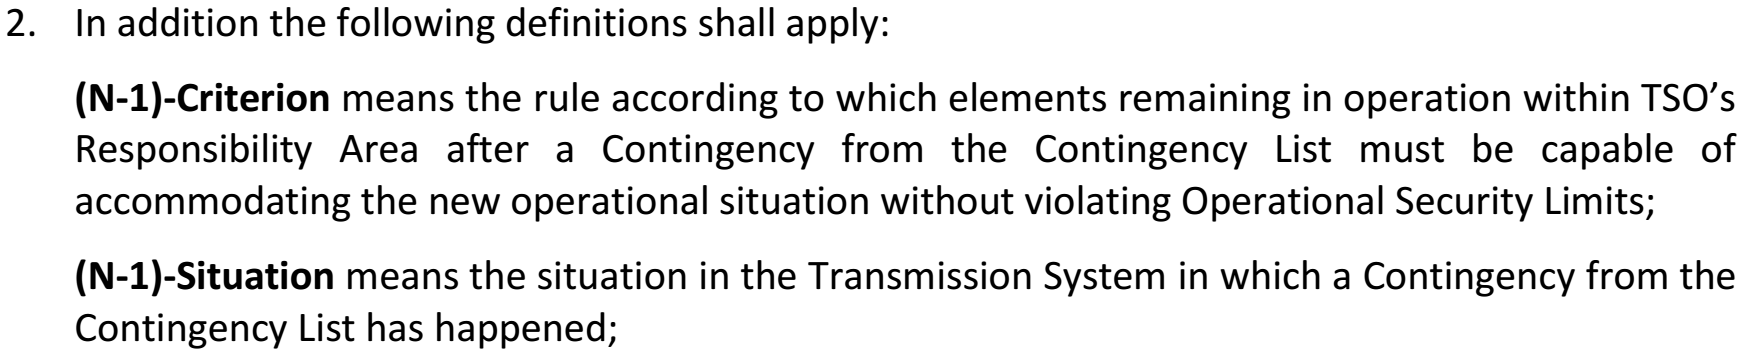
\includegraphics[width=0.9\textwidth]{Figs/N-1_definition.png}\\
In practice, the contingency list contains all single outages and some critical double contingencies (such as double-circuit overhead lines).
\end{block}
\end{frame}

\begin{frame}
  \frametitle{N-1 and N-2 contingencies}
  \begin{columns}
\begin{column}{0.45\textwidth}
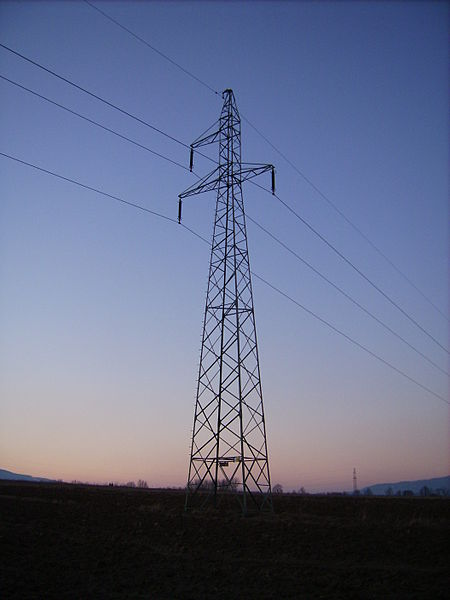
\includegraphics[width=\textwidth]{Figs/SingleCircuit-3phase.JPG}\\
Single-circuit = N-1 contingency
\end{column}
\begin{column}{0.45\textwidth}
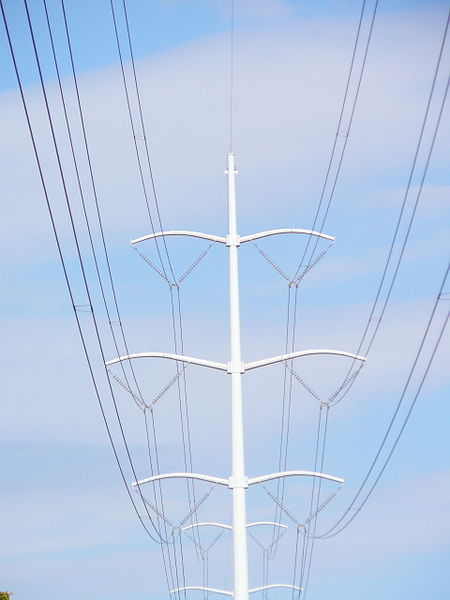
\includegraphics[width=\textwidth]{Figs/DoubleCircuit-3phase.JPG}\\
Double-circuit = N-2 contingency, still included in the contingency list.
\end{column}
  \end{columns}
\end{frame}

\begin{frame}
\frametitle{Security constraints - a summary}
\begin{columns}
\begin{column}{0.5\textwidth}
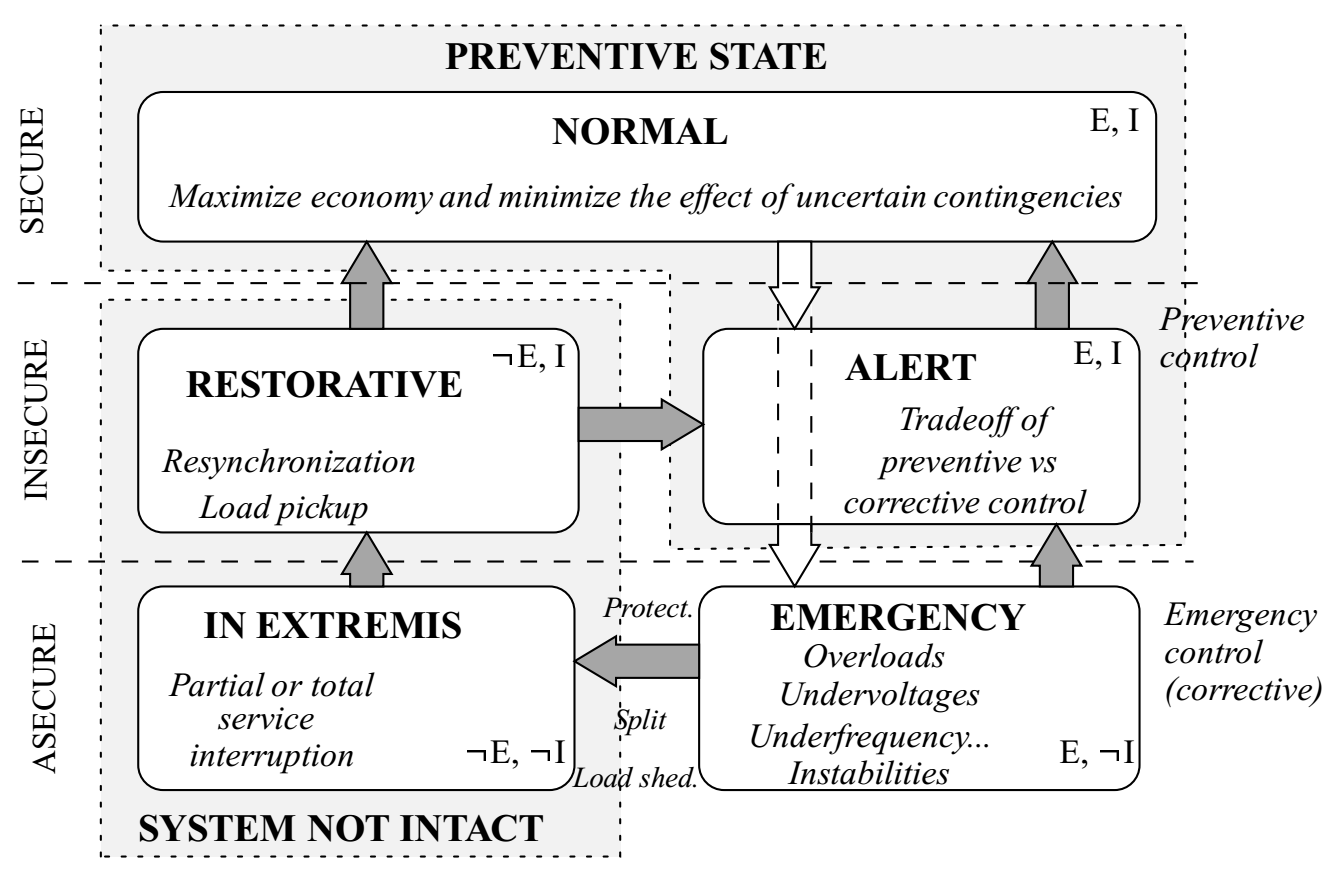
\includegraphics[width=\textwidth]{Figs/FinkCarlsen_SecurityDiagram_trimmed.png}
\end{column}
\begin{column}{0.5\textwidth}
In normal operations, a TSO's responsibility is to enforce the following constraints:
\begin{itemize}
\item Short-circuit constraints
\item Frequency limits
\item \emph{Bus voltage constraints}
\item \emph{Thermal limits}
\item \emph{Stability limits}
\end{itemize}
for all contingencies in its \underline{contingency list}.
\end{column}
\end{columns}
\end{frame}

\begin{frame}
  \frametitle{Question}
  \begin{columns}
    \begin{column}{0.5\textwidth}
    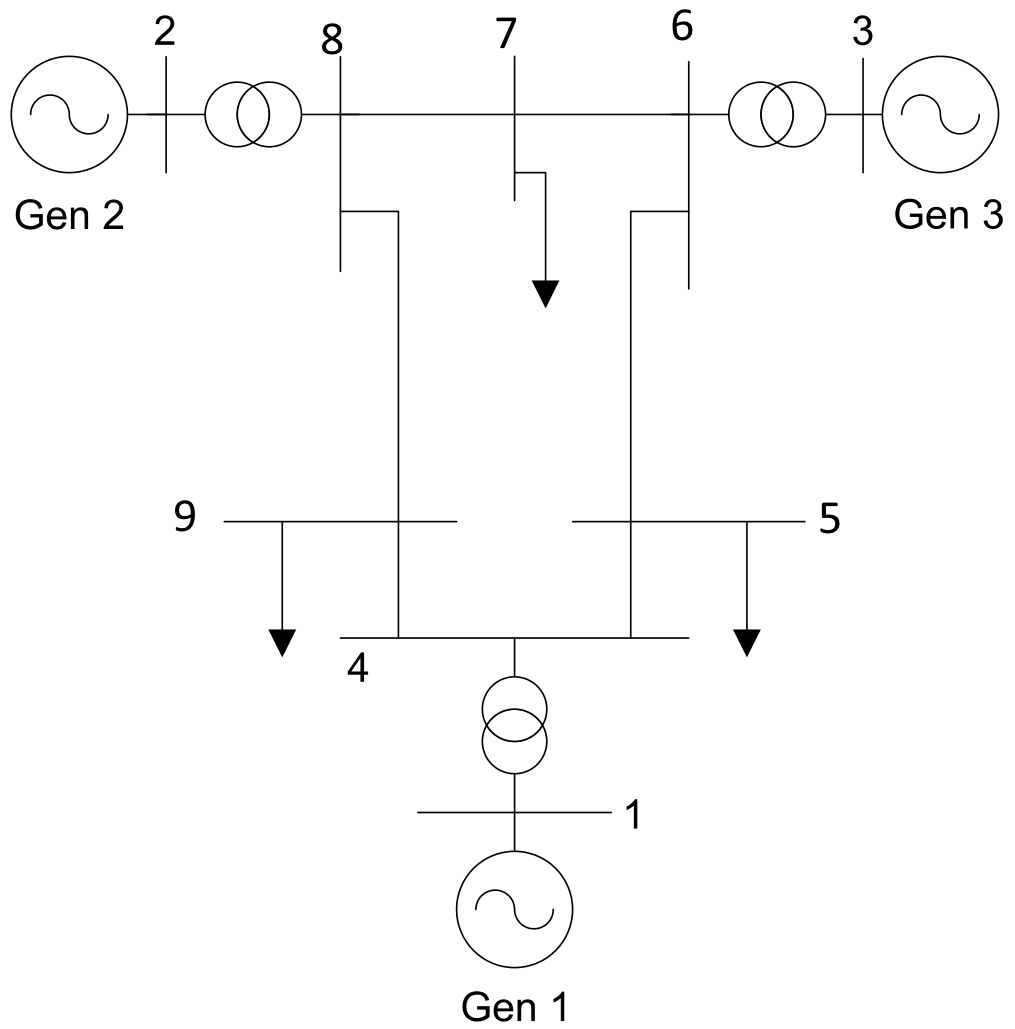
\includegraphics[width=\textwidth]{Figs/ieee9.png}\\  
    \end{column}
    \begin{column}{0.5\textwidth}
\begin{itemize}
\item What contingencies are included in the N-1 contingency list of this system?
\end{itemize}      
    \end{column}
  \end{columns}
\end{frame}

\section[SCOPF]{Security constrained optimal power flow (SCOPF)}
\begin{frame}
  \frametitle{Examples of problems a TSO faces}
\textbf{Day-ahead problem}
  \begin{itemize}
  \item Do the market generation and consumption plans comply with the security requirements? $\Leftrightarrow$ contingency analyses
  \item What actions must be taken \underline{now} if they do not? $\Leftrightarrow$ SCOPF.
  \end{itemize}

\textbf{Real-time operation}
  \begin{itemize}
  \item Does the current system comply with the security requirements? $\Leftrightarrow$ contingency analyses.
  \item What actions must be taken \underline{now} if they do not? $\Leftrightarrow$ SCOPF.
  \end{itemize}

\textbf{SCOPF is one possible tool (not the only one) to answer these questions}
\end{frame}

\begin{frame}
  \frametitle{SCOPF for real-time decision making}
\begin{columns}
\begin{column}{0.5\textwidth}
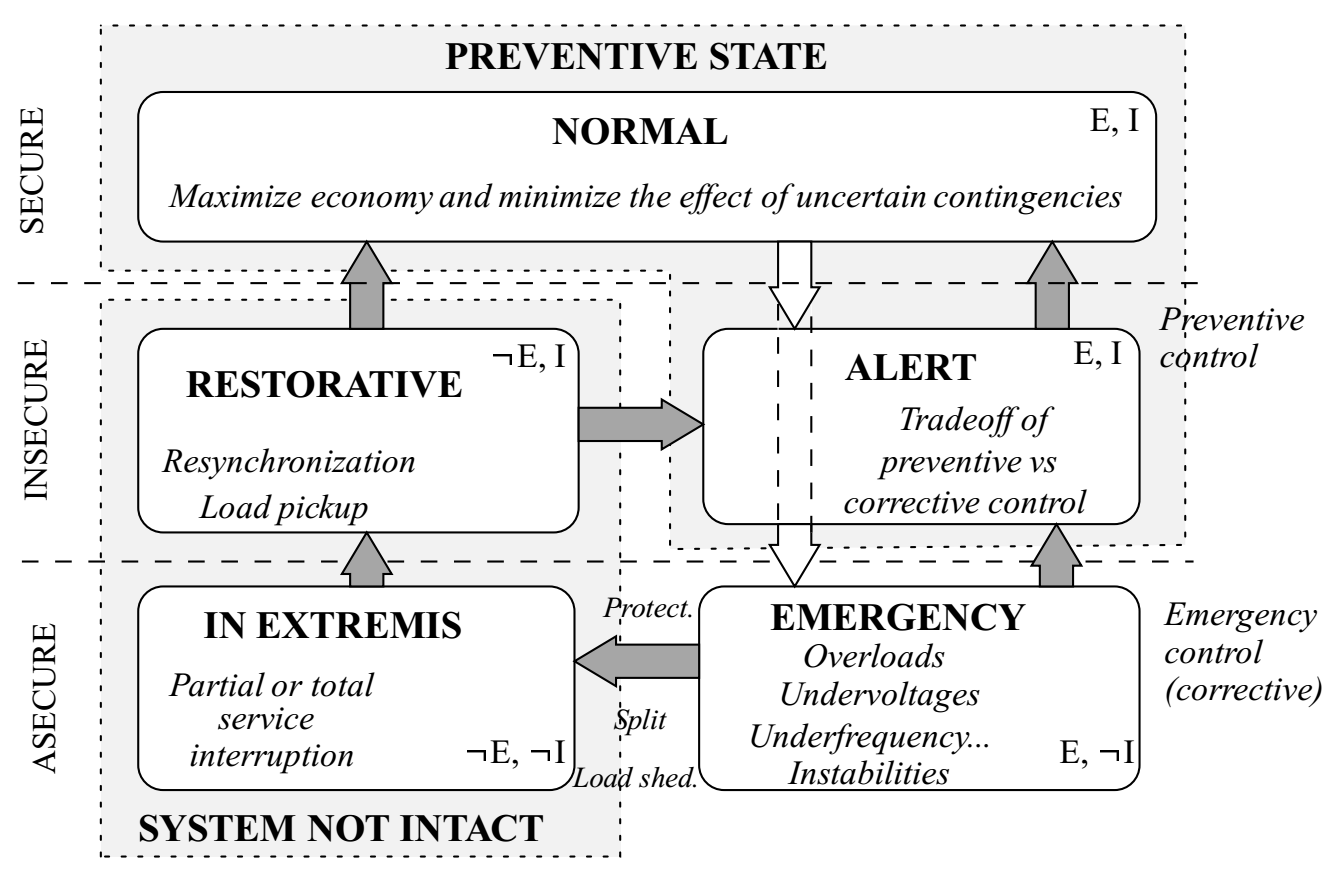
\includegraphics[width=\textwidth]{Figs/FinkCarlsen_SecurityDiagram_trimmed.png}
\end{column}
\begin{column}{0.5\textwidth}
\only<1>{
\underline{Assumption}: no contingency has happened yet.

What is our ``problem formulation''?}
\only<2>{Power system problem: 
  \begin{itemize}
  \item are we in the normal or alert state? $\Rightarrow$ \uline{contingency analyses}
  \item If we are in the alert state, what actions should we take \underline{now}? $\Rightarrow$ SCOPF
  \end{itemize}
}
\only<3>{\begin{block}{Formulating the problem}
We need to decide:
    \begin{itemize}
    \item What is the contingency list? 
    \item What are the security constraints? 
    \item What are available actions if necessary?
    \item What are the costs of these actions?
    \end{itemize}
  \end{block}}
\end{column}
\end{columns}
\end{frame}

\begin{frame}
  \frametitle{Contingency analysis - Illustration}
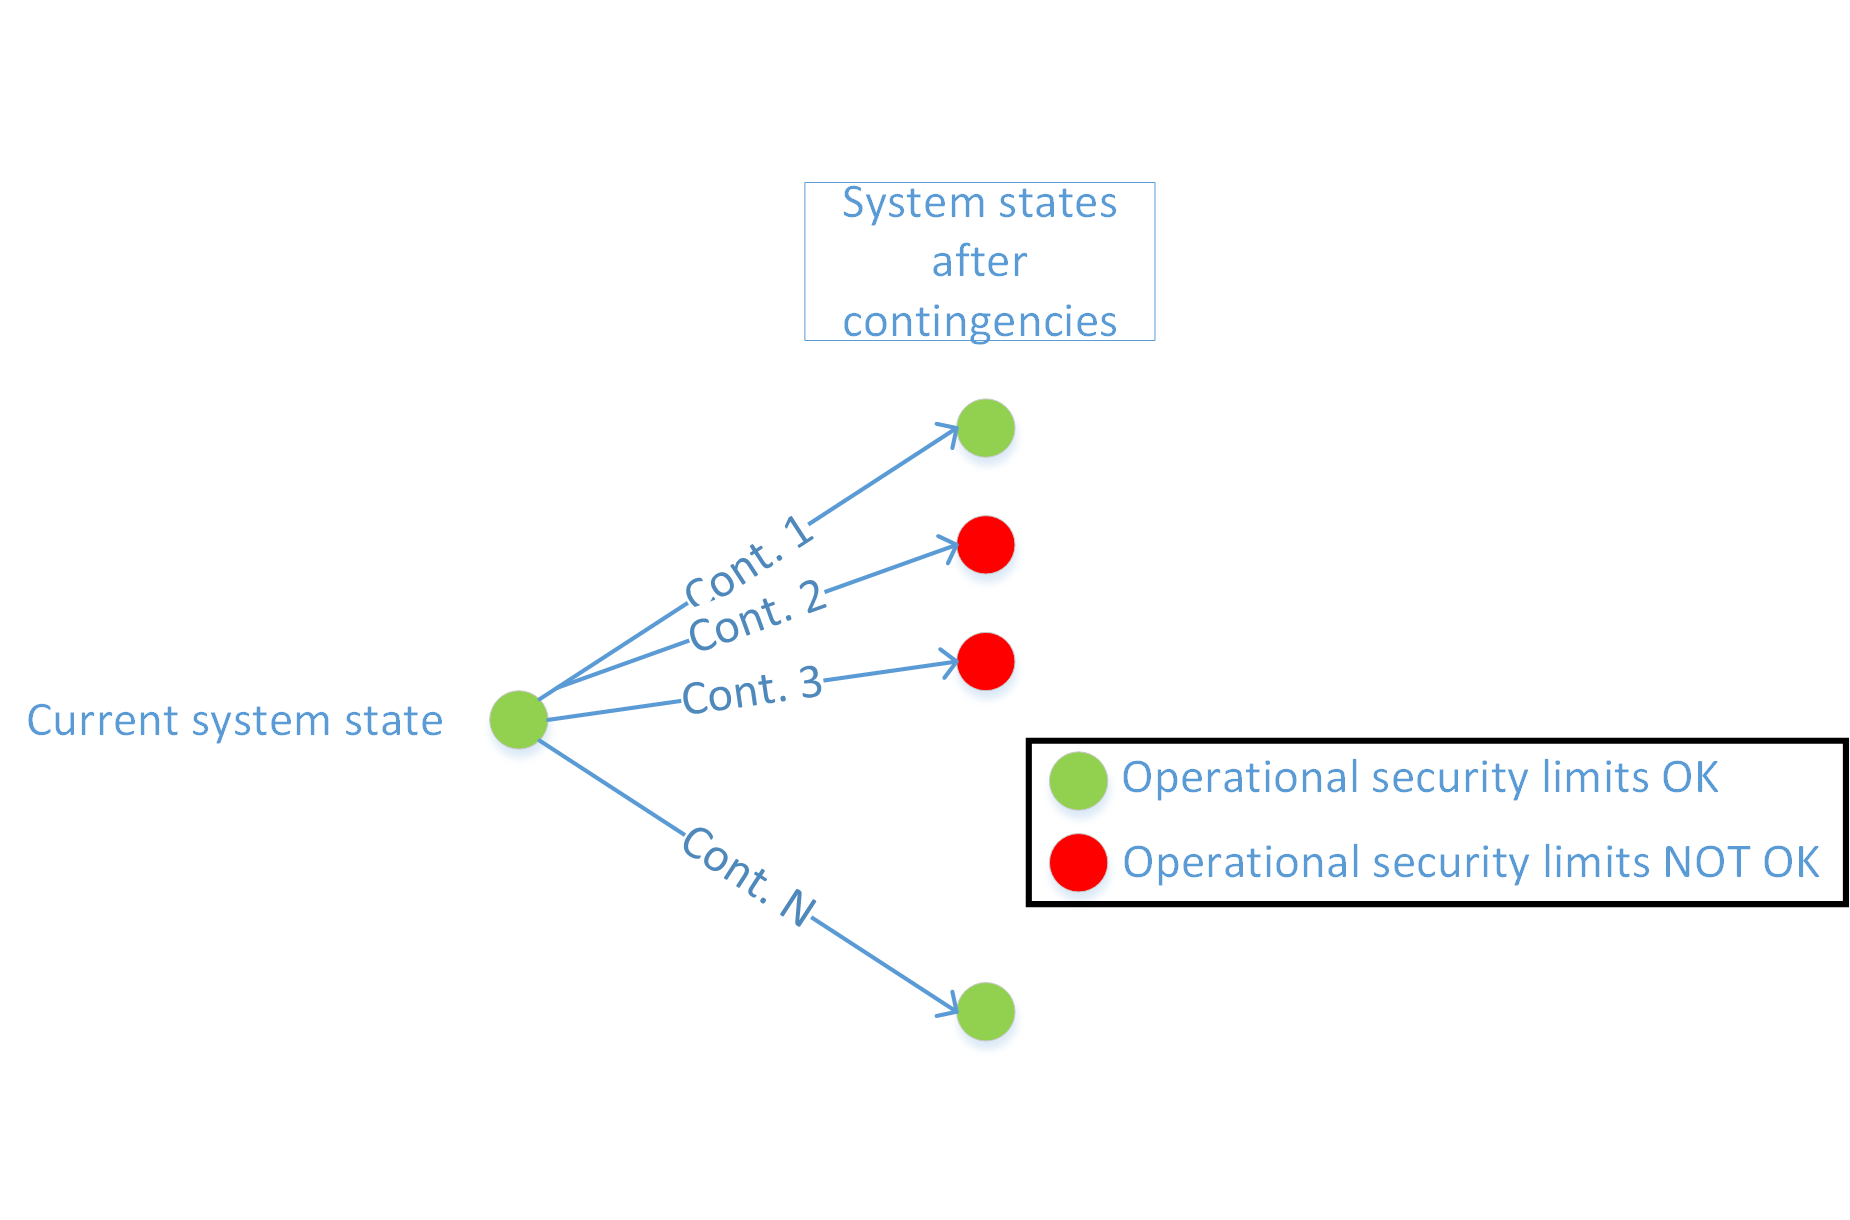
\includegraphics[width=0.9\textwidth]{Figs/Event-tree-cont-ana.png}
\end{frame}


\begin{frame}
  \frametitle{Example}
  \begin{columns}
    \begin{column}{0.5\textwidth}
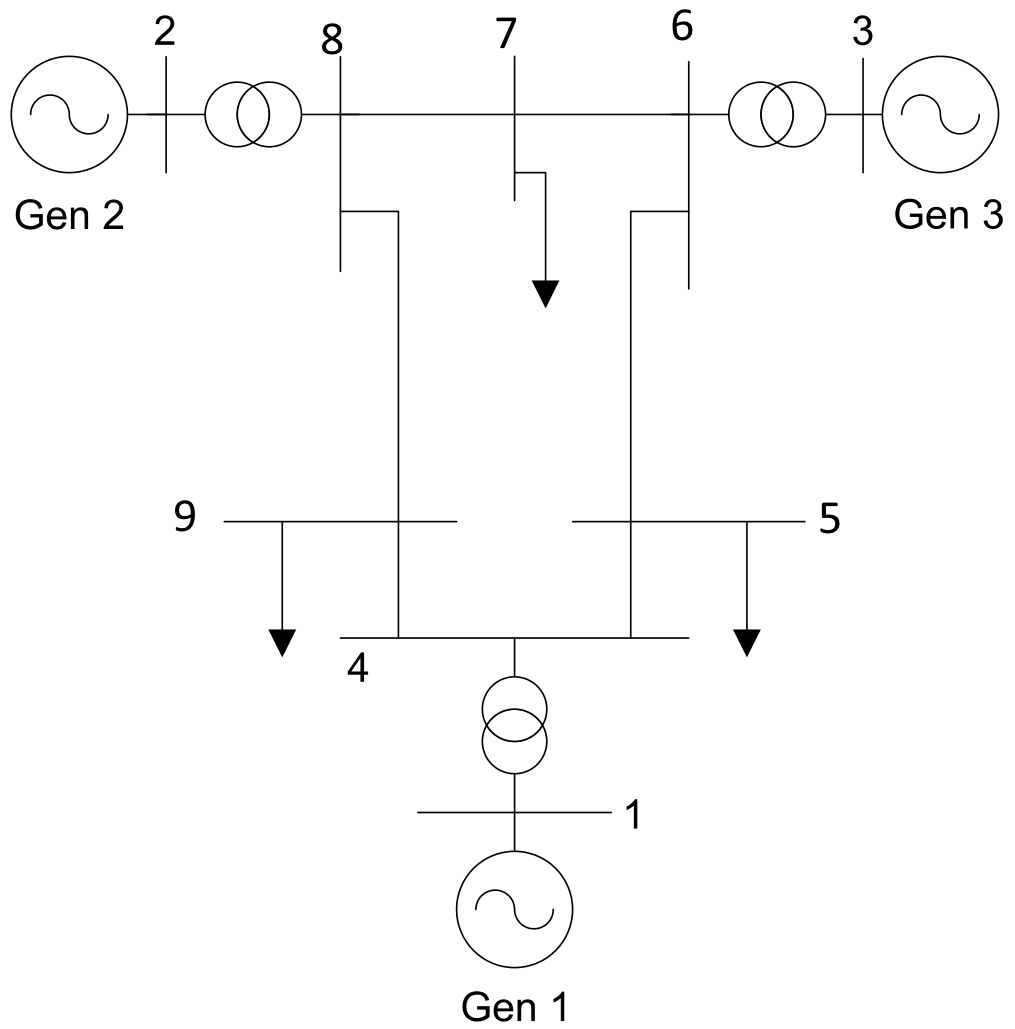
\includegraphics[width=\textwidth]{Figs/ieee9.png}
    \end{column}
    \begin{column}{0.5\textwidth}
      \begin{itemize}
      \item Contingency list: N-1 contingency list
      \item Security constraints: Voltage limits and line ratings
      \item Actions: Re-dispatch of generators
      \item Cost: Re-dispatch cost
      \end{itemize}
    \end{column}
  \end{columns}
\end{frame}

\begin{frame}
  \frametitle{Example - contingency analysis}
  \begin{columns}
    \begin{column}{0.5\textwidth}
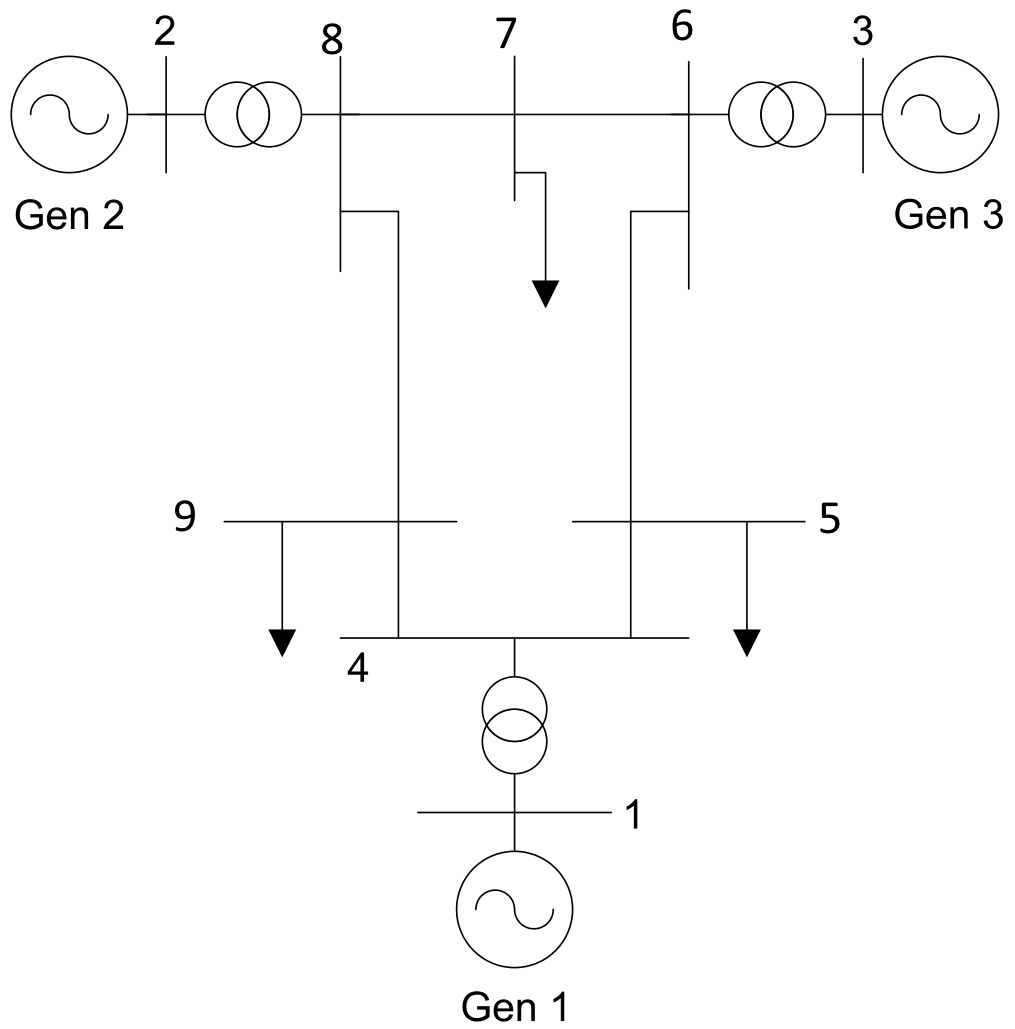
\includegraphics[width=\textwidth]{Figs/ieee9.png}
    \end{column}
    \begin{column}{0.5\textwidth}
For all contingencies in the contingency list:
      \begin{itemize}
      \item Apply contingency.
      \item Simulate system response. (How?)
      \item Check the security constraints.
      \end{itemize}
\only<1>{See example in MATPOWER.}
\only<2>{\textbf{\color{red} System in alert state} $\Rightarrow$ actions must be taken.}
    \end{column}
  \end{columns}
\end{frame}


\begin{frame}
  \frametitle{Preventive SCOPF}
  \begin{align}
\label{eq:2}\tag{P-SCOPF}
    \begin{split}
    \min_{u_0,x_c} \; & C(u_0) \\
    \text{subject to} \; & g_c(x_c,u_0) = 0, \; c = 0,\ldots,n_c \\
    & h_c(x_c,u_0) \leq h_c^{\text{max}}, \; c = 0,\ldots,n_c
    \end{split}
  \end{align}
  \begin{itemize}
  \item $c=1,\ldots,n_c$ are contingencies, $c=0$ is the pre-contingency case.
  \item $x_c$ is the state of the system (typically voltage angles and magnitudes), after contingency $c$ occurs.
  \item $u_0$ are the preventive actions.
  \item $g_c$ are the power flow equations.
  \item $h_c^\text{max}$ are the security limits.
  \end{itemize}
The optimal solution $u_0^{*}$ is the cheapest set of preventive actions that enforces the security limits for the considered contingency list.
\end{frame}

\begin{frame}
  \frametitle{Preventive SCOPF - discussion}
  \begin{align}
\label{eq:2}\tag{P-SCOPF}
    \begin{split}
    \min_{u_0,x_c} \; & C(u_0) \\
    \text{subject to} \; & g_c(x_c,u_0) = 0, \; c = 0,\ldots,n_c \\
    & h_c(x_c,u_0) \leq h_c^{\text{max}}, \; c = 0,\ldots,n_c
    \end{split}
  \end{align}
  \begin{itemize}
  \item The control actions $u_0$ are applied \underline{now} 
  \item They apply to \underline{all} pre- and post-contingency systems, thereby the name ``preventive''
  \item We take actions before the contingencies occur.
  \item We take necessary actions \underline{now} so that the security limits are fulfilled even if one of the contingencies $c$ occurs.
  \item \underline{Note:} we do not know what happens with contingencies outside the contingency list (maybe secure, maybe not).
  \item \underline{Limitation}: P-SCOPF does not consider the possibility of using corrective actions after contingencies occur.
  \end{itemize}
\end{frame}

\begin{frame}
  \frametitle{Preventive action - illustration}
\only<1>{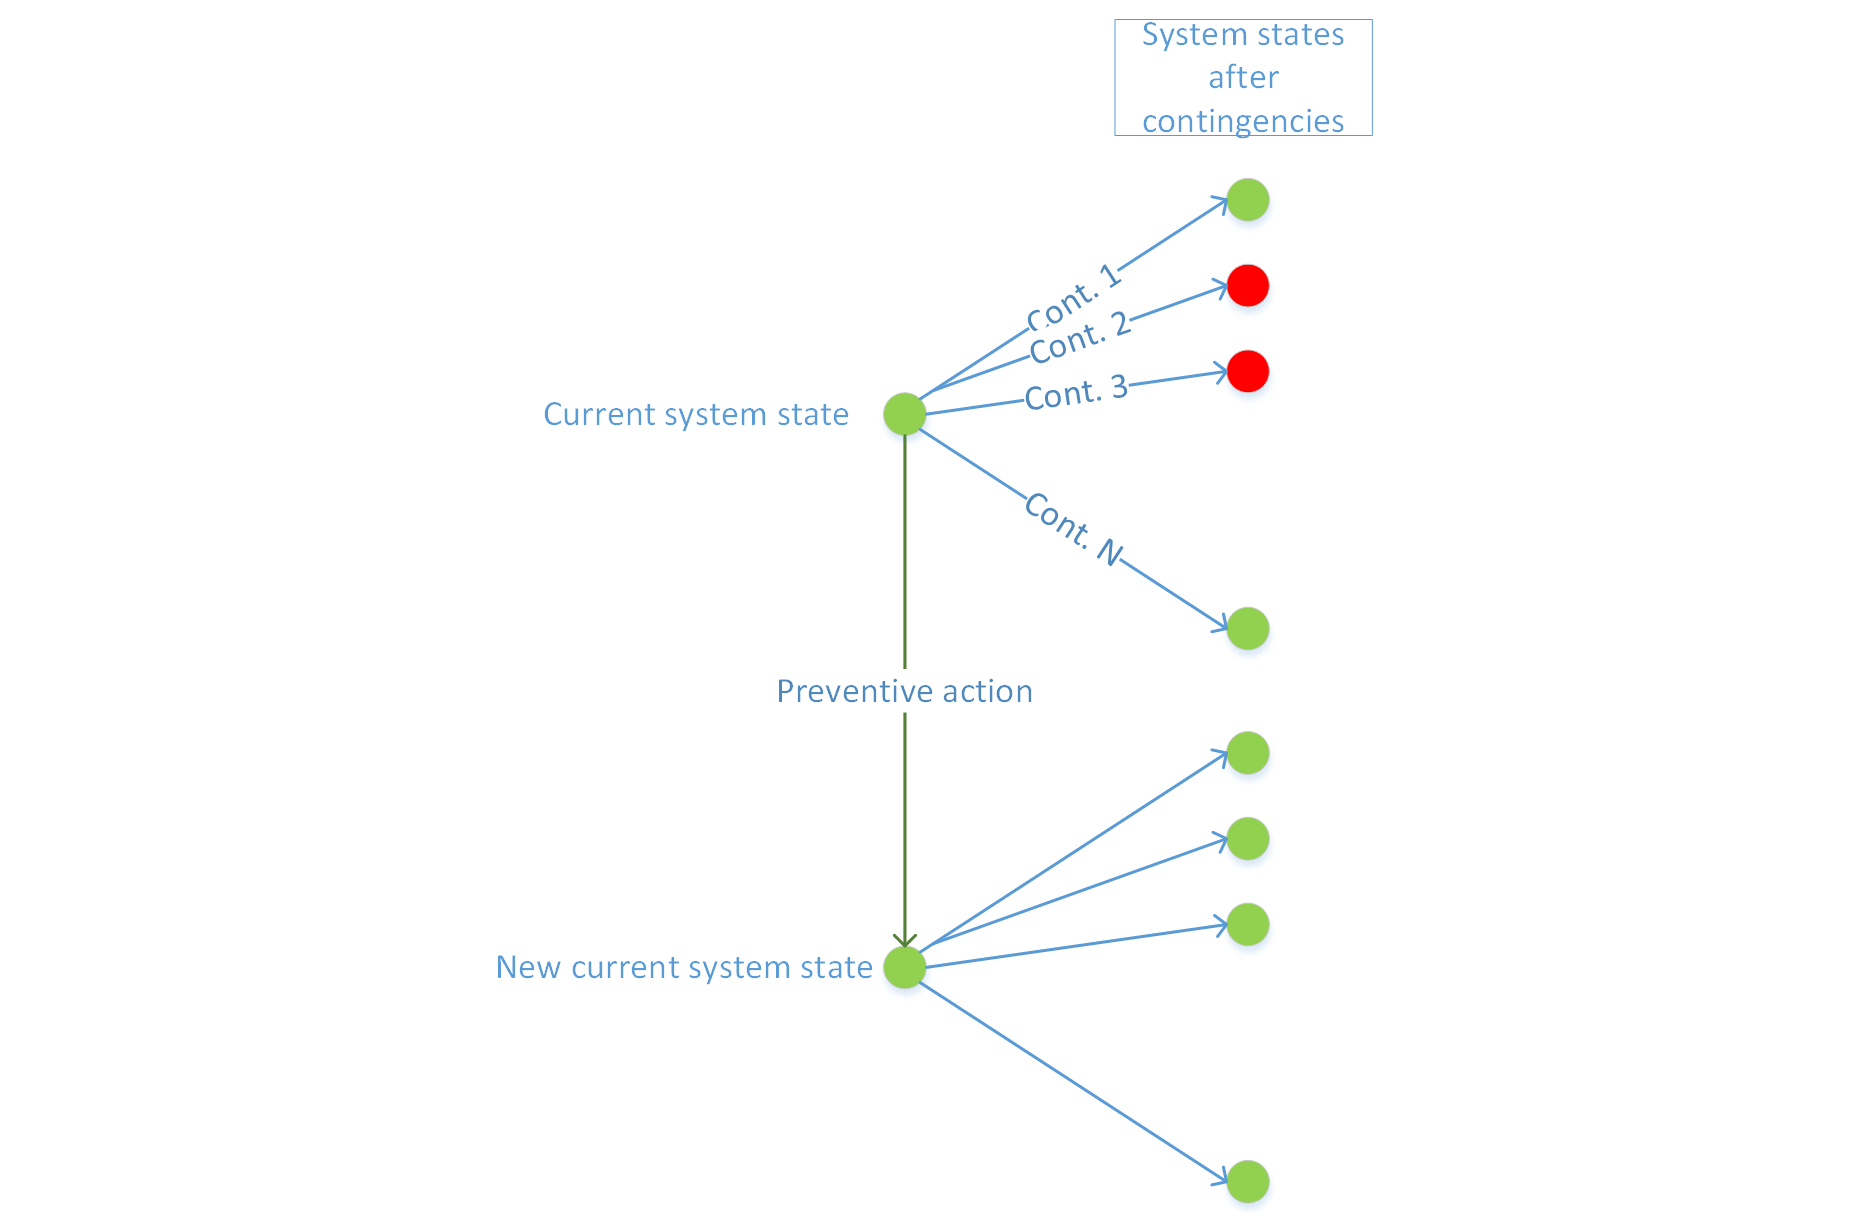
\includegraphics[width=1\textwidth]{Figs/Event-tree-prev-actions.png}}
\only<2>{This can also happen if contingencies are not explicitly/properly considered when finding preventive actions!\\ 
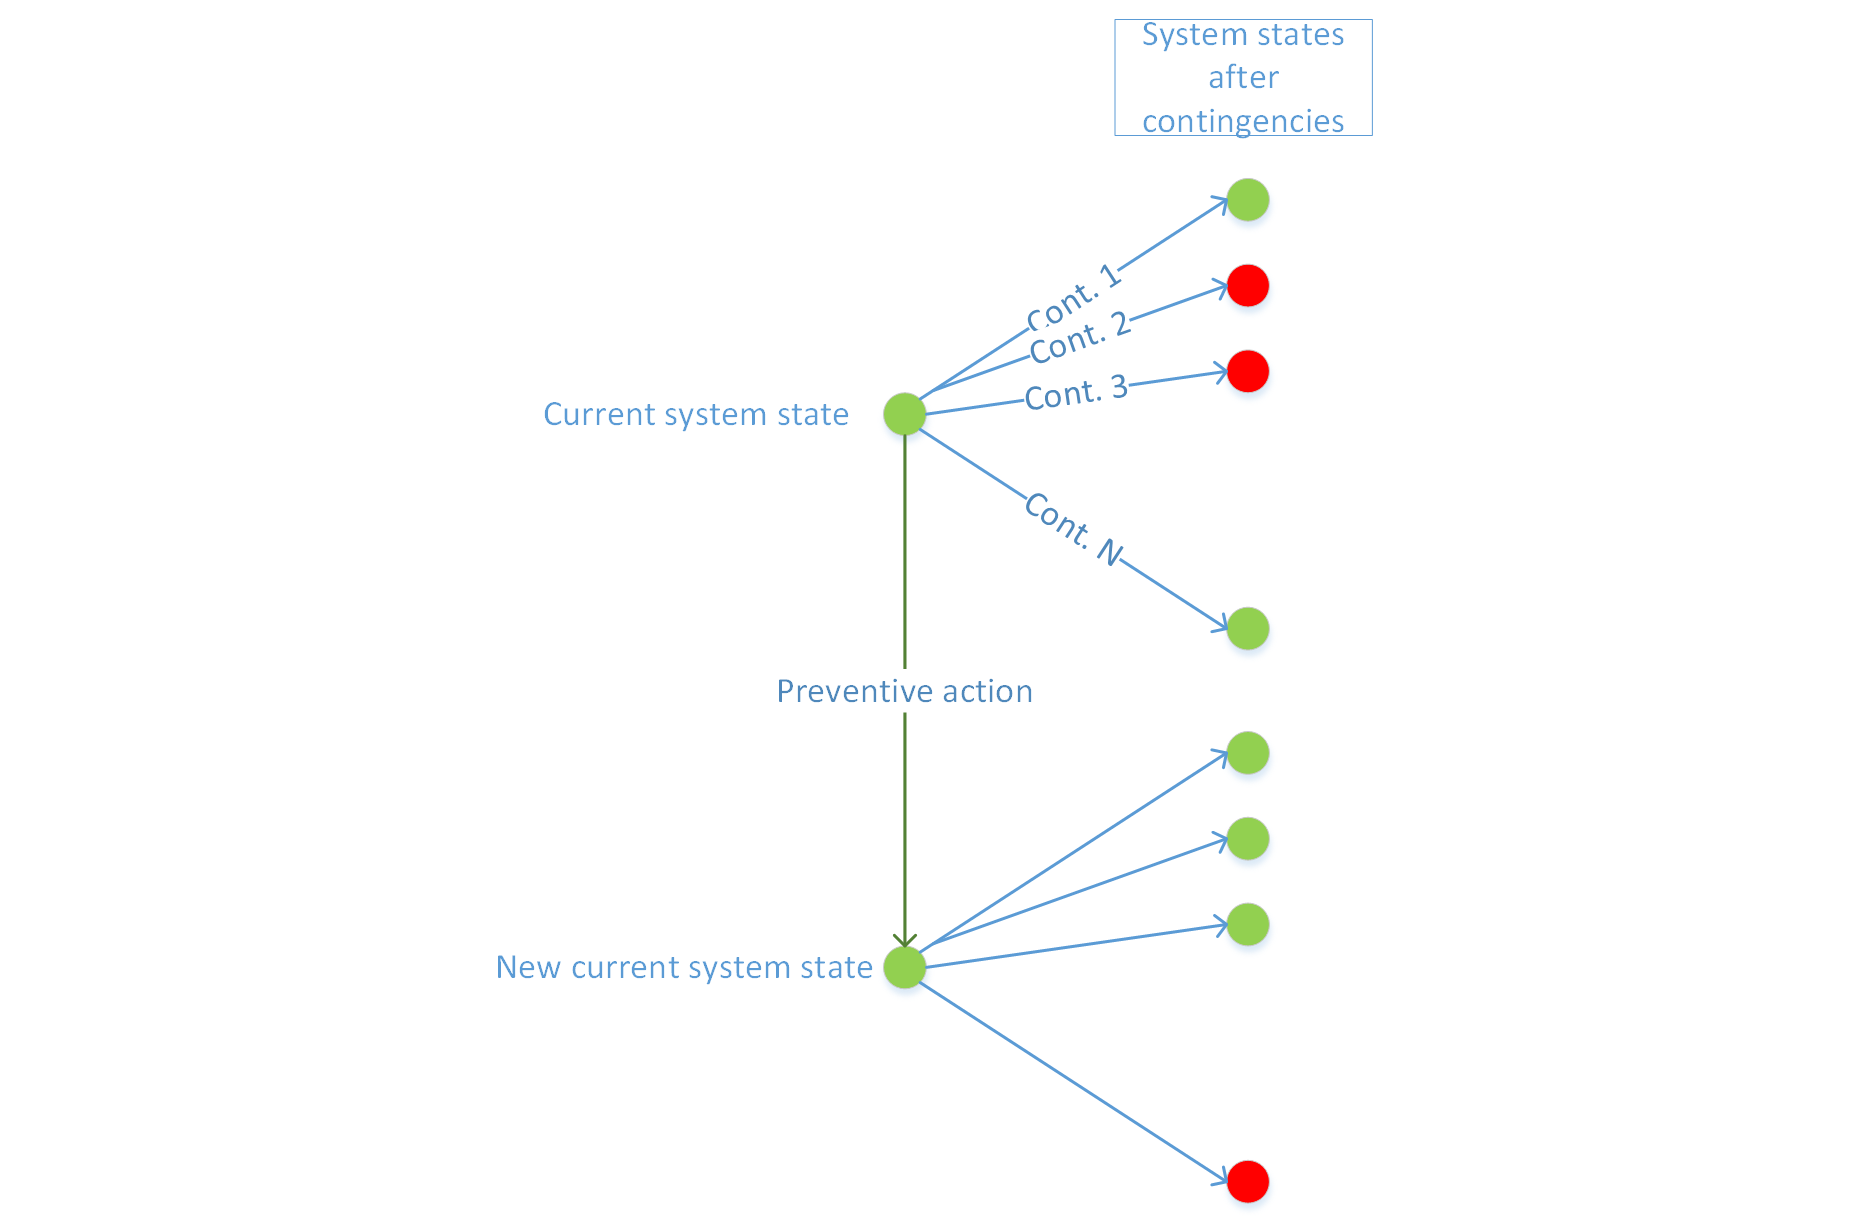
\includegraphics[width=1\textwidth]{Figs/Event-tree-wrong-prev-actions.png}}
\end{frame}

\begin{frame}
  \frametitle{Examples}
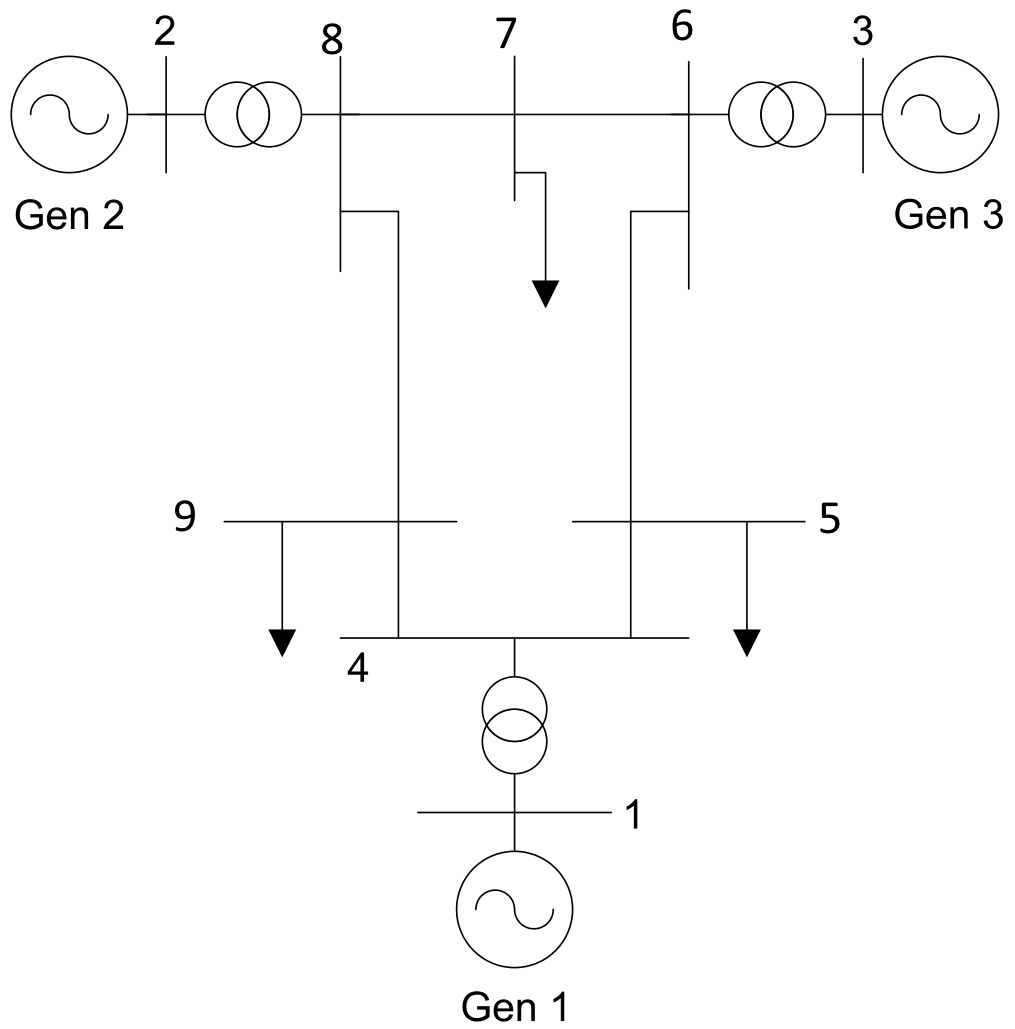
\includegraphics[width=0.6\textwidth]{Figs/ieee9.png}\\
See examples in MATPOWER
\end{frame}

\begin{frame}
  \frametitle{Preventive-corrective SCOPF}
  \begin{align}
  \tag{PC-SCOPF}
    \begin{split}
    \min_{x_0,x_c,u_0,u_c} \; & C(u_0) \\
    \text{subject to} \; & g_0(x_0,u_0) = 0, \; \\
    & g_c(x_c,u_c) = 0, \; c = 1,\ldots,n_c \\
    & h_0(x_0,u_0) \leq h_0^{\text{max}}, \\
    & h_c(x_c,u_c) \leq h_c^{\text{max}}, \; c = 1,\ldots,n_c \\
    & \norm{u_c - u_0} \leq \Delta u_c^{max}
    \end{split}
  \end{align}
  \begin{itemize}
  \item $u_c$ are the corrective controls. Note that they apply only in the corresponding contingency $c$.
  \item As many different $u_c$ as contingencies.
  \item The last equation limits the possible range of corrective actions. For example: $\Delta u_c^\text{max} = T_c R$, with $T_c$ the time available to corrective control to react (say 10 minutes), and $R$ the ramp rates of power plants (say 20 MW/min).
  \end{itemize}
\end{frame}

\begin{frame}
  \frametitle{Preventive-corrective SCOPF - discussion}
  \begin{align}
  \tag{PC-SCOPF}
    \begin{split}
    \min_{x_0,x_c,u_0,u_c} \; & C(u_0) \\
    \text{subject to} \; & g_0(x_0,u_0) = 0, \; \\
    & g_c(x_c,u_c) = 0, \; c = 1,\ldots,n_c \\
    & h_0(x_0,u_0) \leq h_0^{\text{max}}, \\
    & h_c(x_c,u_c) \leq h_c^{\text{max}}, \; c = 1,\ldots,n_c \\
    & \norm{u_c - u_0} \leq \Delta u_c^{max}
    \end{split}
  \end{align}
  \begin{itemize}
  \item $u_0$ is now the cheapest set of preventive actions that enforces security limits, \underline{knowing that corrective actions are available}
  \item Remember, corrective actions $u_k$ \underline{are not taken now}.
  \item Preventive actions $u_0$ affect all pre- and post-contingency systems. The corrective action $u_c$ affects \underline{only} the system after contingency $c$.
  \end{itemize}
\end{frame}

\begin{frame}
  \frametitle{Preventive and corrective actions - Illustration}
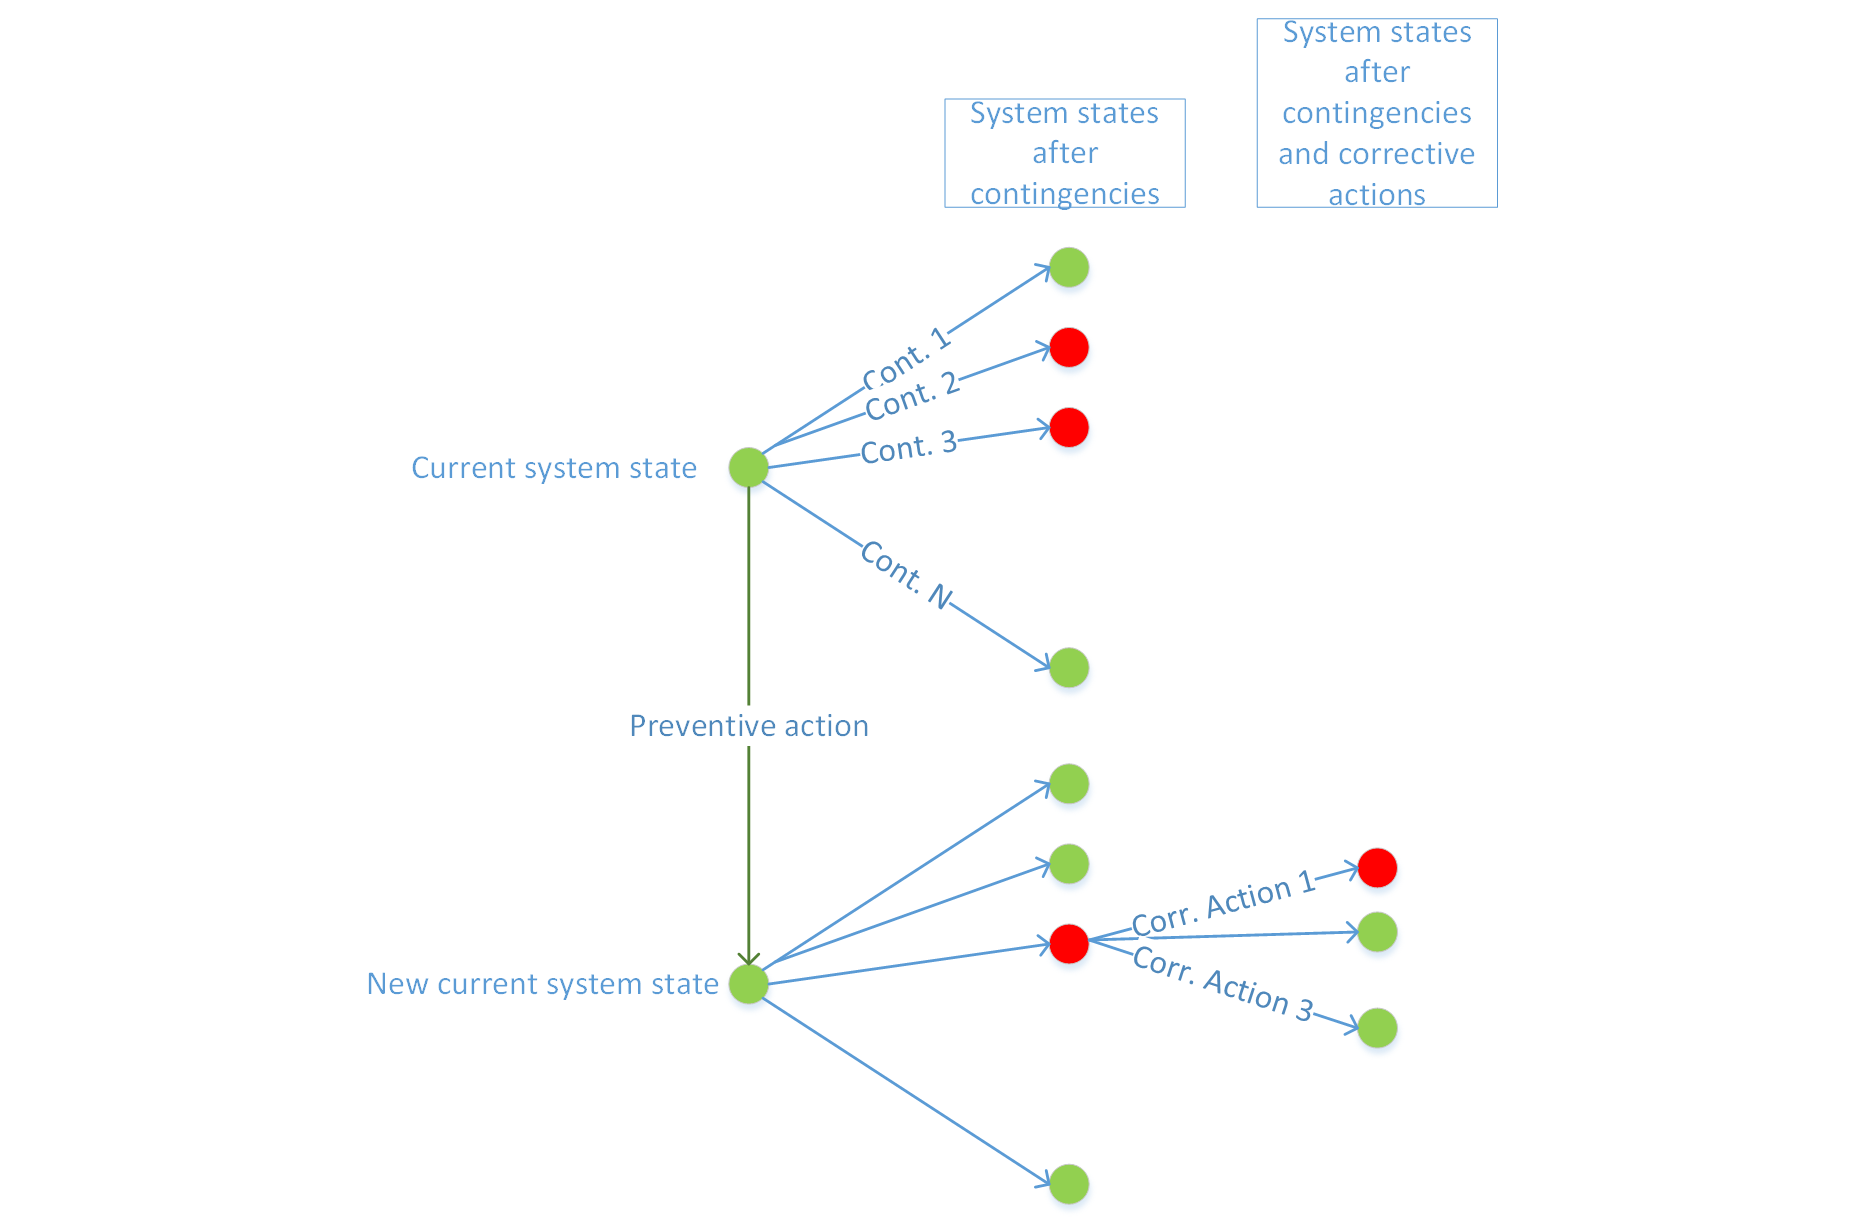
\includegraphics[width=\textwidth]{Figs/Event-tree-prev-corr-actions.png}
\end{frame}

\begin{frame}
  \frametitle{Example}
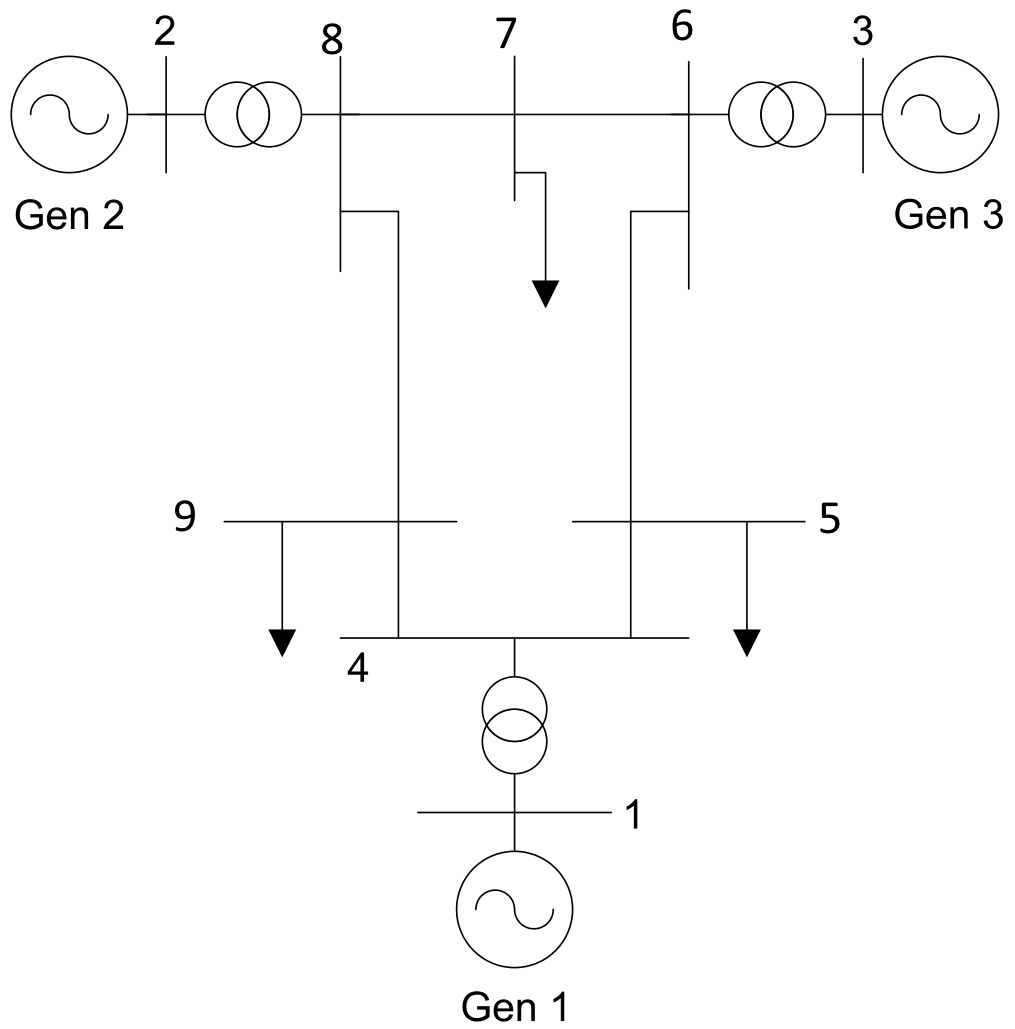
\includegraphics[width=0.6\textwidth]{Figs/ieee9.png}\\
See examples in MATPOWER  
\end{frame}

\begin{frame}
  \frametitle{Preventive-corrective SCOPF - discussion 2}
  \begin{align}
  \tag{PC-SCOPF}
    \begin{split}
    \min_{x_0,x_c,u_0,u_c} \; & C(u_0) \\
    \text{subject to} \; & g_0(x_0,u_0) = 0, \; \\
    & g_c(x_c,u_c) = 0, \; c = 1,\ldots,n_c \\
    & h_0(x_0,u_0) \leq h_0^{\text{max}}, \\
    & h_c(x_c,u_c) \leq h_c^{\text{max}}, \; c = 1,\ldots,n_c \\
    & \norm{u_c - u_0} \leq \Delta u_c^{max}
    \end{split}
  \end{align}
What is the problem with this formulation? (Hint: corrective controls react in, say, 10 minutes)
\end{frame}

\begin{frame}
  \frametitle{Corrective actions and short-term limits}
From the network code on operational security, Article 8:
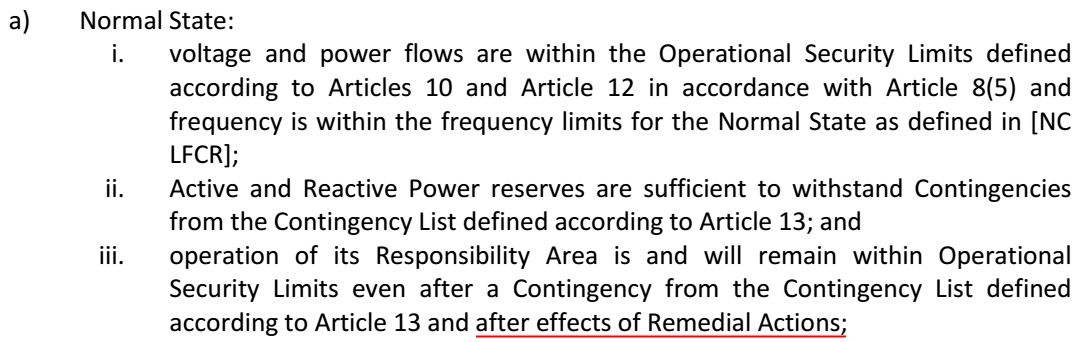
\includegraphics[width=0.6\textwidth]{Figs/NormalStateRA.png}\\
and Article 12 \\
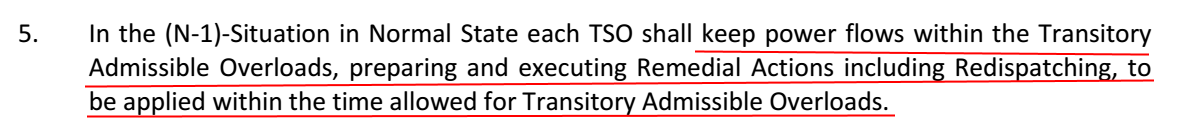
\includegraphics[width=0.6\textwidth]{Figs/RA_ShortTermLimits.png}
\begin{itemize}
\item Remember: emergency limits can be sustained for a short while (say 10-15 minutes)
\item If the flow on a line is larger than the continuous limit but smaller than the emergency limits $\Leftrightarrow$ ``Transitory admissible overloads''
\item TSOs have a certain amount of time (10-15 minutes) to implement corrective actions.
\end{itemize}
\scriptsize Preventive actions = pre-fault remedial actions; corrective actions = post-fault remedial actions.
\end{frame}



\begin{frame}
  \frametitle{Improved preventive-corrective SCOPF}
  \begin{align}
  \tag{PC-SCOPF}
    \begin{split}
    \min_{x_0,x_c,u_0,u_c} \; & C(u_0) \\
    \text{subject to} \; & g_0(x_0,u_0) = 0, \; \\
    & g_c(x_c,u_c) = 0, \; c = 1,\ldots,n_c \\
    & h_0(x_0,u_0) \leq h_0^{\text{max},LT}, \\
    & h_c(x_c,u_0) \leq h_c^{\text{max},ST}, \; c = 1,\ldots,n_c \\
    & h_c(x_c,u_c) \leq h_c^{\text{max},LT}, \; c = 1,\ldots,n_c \\
    & \norm{u_c - u_0} \leq \Delta u_c^{max}
    \end{split}
  \end{align}
  \begin{itemize}
  \item $h_c^{\text{max},ST}$ and $h_c^{\text{max},LT}$ are the emergency and continuous ratings.
  \item Preventive actions ensure that the post-contingency systems are within the emergency limits while corrective actions can be called upon to bring the system back within the continuous limits.
  \end{itemize}
\end{frame}

\begin{frame}
  \frametitle{Improved preventive-corrective SCOPF}
  \begin{align}
  \tag{PC-SCOPF}
    \begin{split}
    \min_{x_0,x_c,u_0,u_c} \; & C(u_0) \\
    \text{subject to} \; & g_0(x_0,u_0) = 0, \; \\
    & g_c(x_c,u_c) = 0, \; c = 1,\ldots,n_c \\
    & h_0(x_0,u_0) \leq h_0^{\text{max},LT}, \\
    & h_c(x_c,u_0) \leq h_c^{\text{max},ST}, \; c = 1,\ldots,n_c \\
    & h_c(x_c,u_c) \leq h_c^{\text{max},LT}, \; c = 1,\ldots,n_c \\
    & \norm{u_c - u_0} \leq \Delta u_c^{max}
    \end{split}
  \end{align}
  \begin{itemize}
  \item Proposed in Capitanescu and Wehenkel (2007), ``Improving the statement of the corrective security-constrained optimal power-flow problem''
  \end{itemize}
\end{frame}

\begin{frame}
  \frametitle{Improved preventive-corrective SCOPF - illustration}
\only<1>{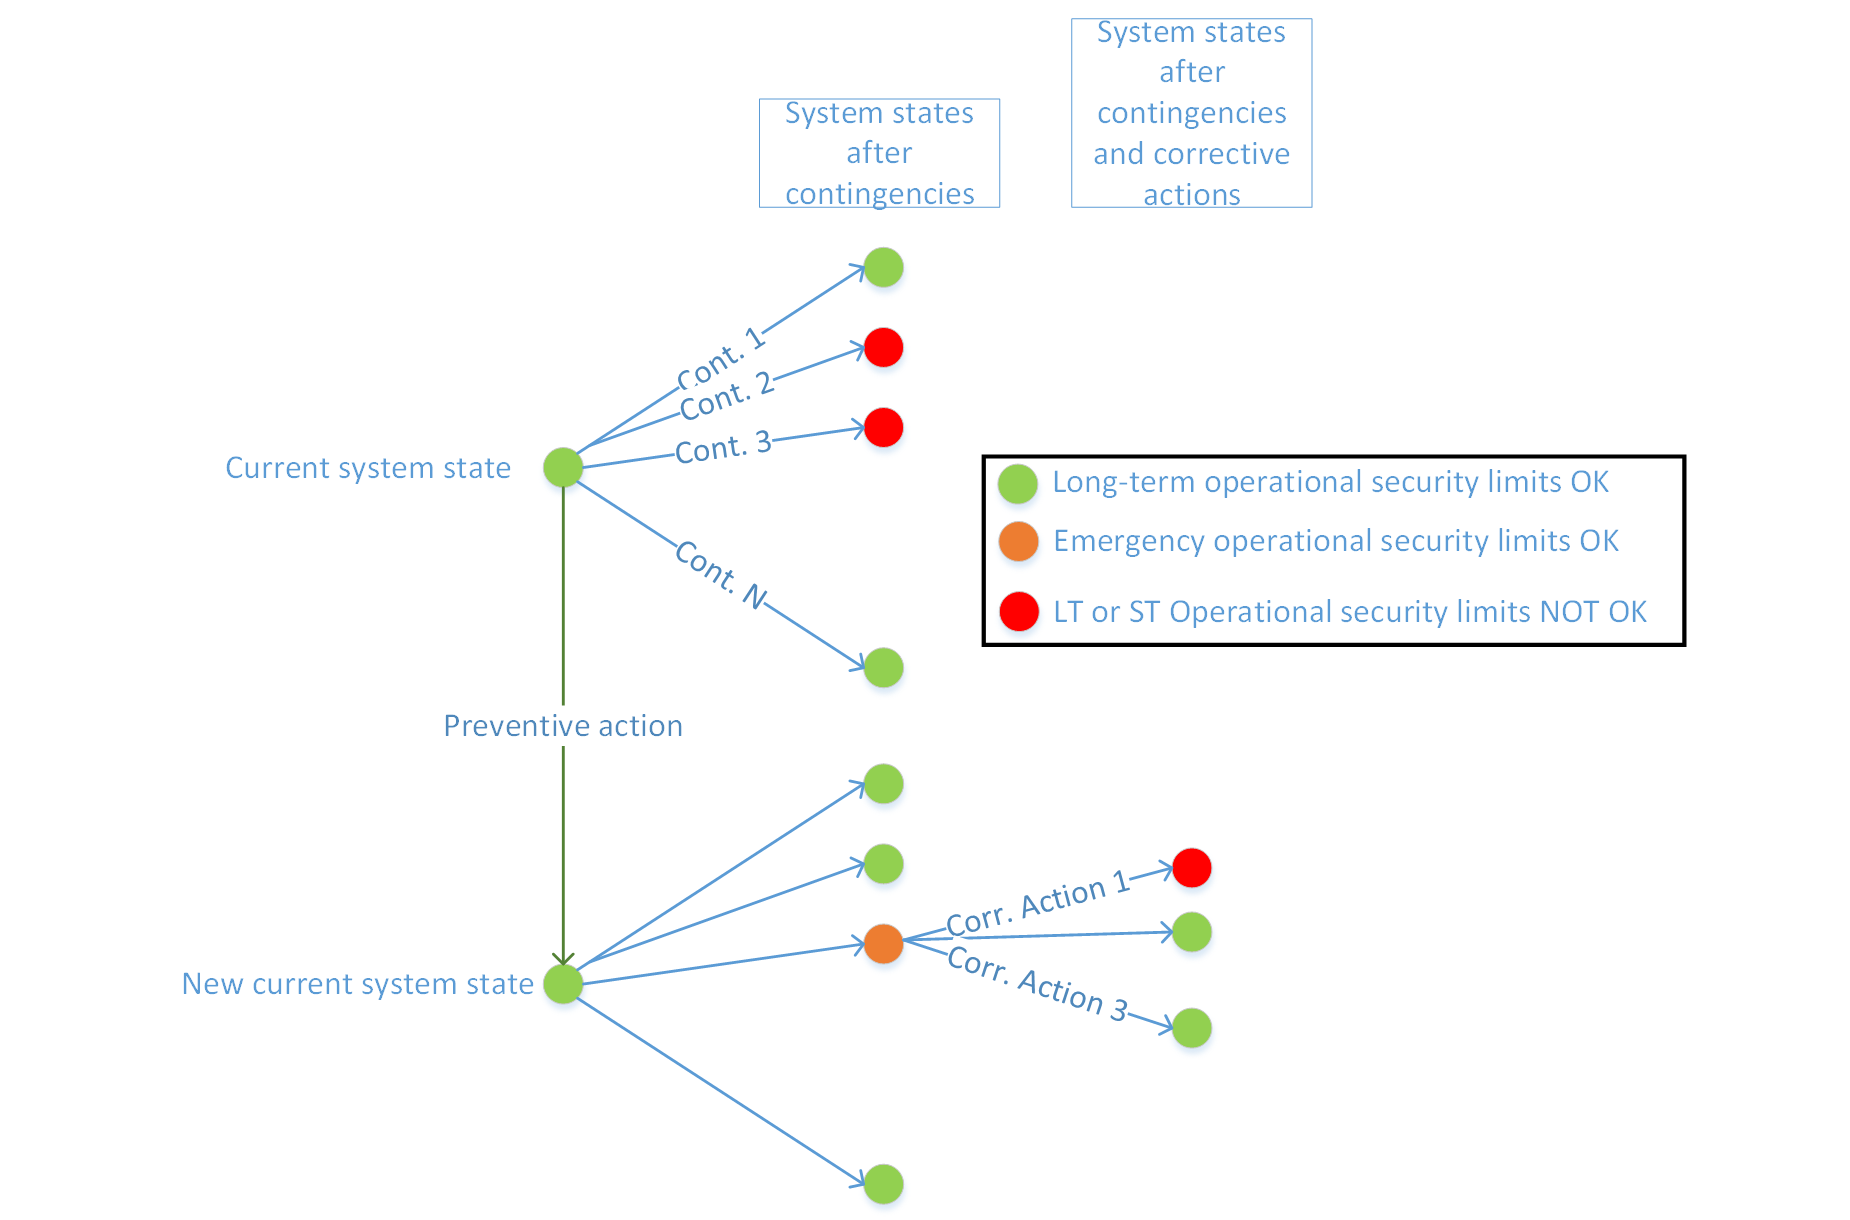
\includegraphics[width=1\textwidth]{Figs/Event-tree-prev-corr-actions-stlt-limits.png}}
\only<2>{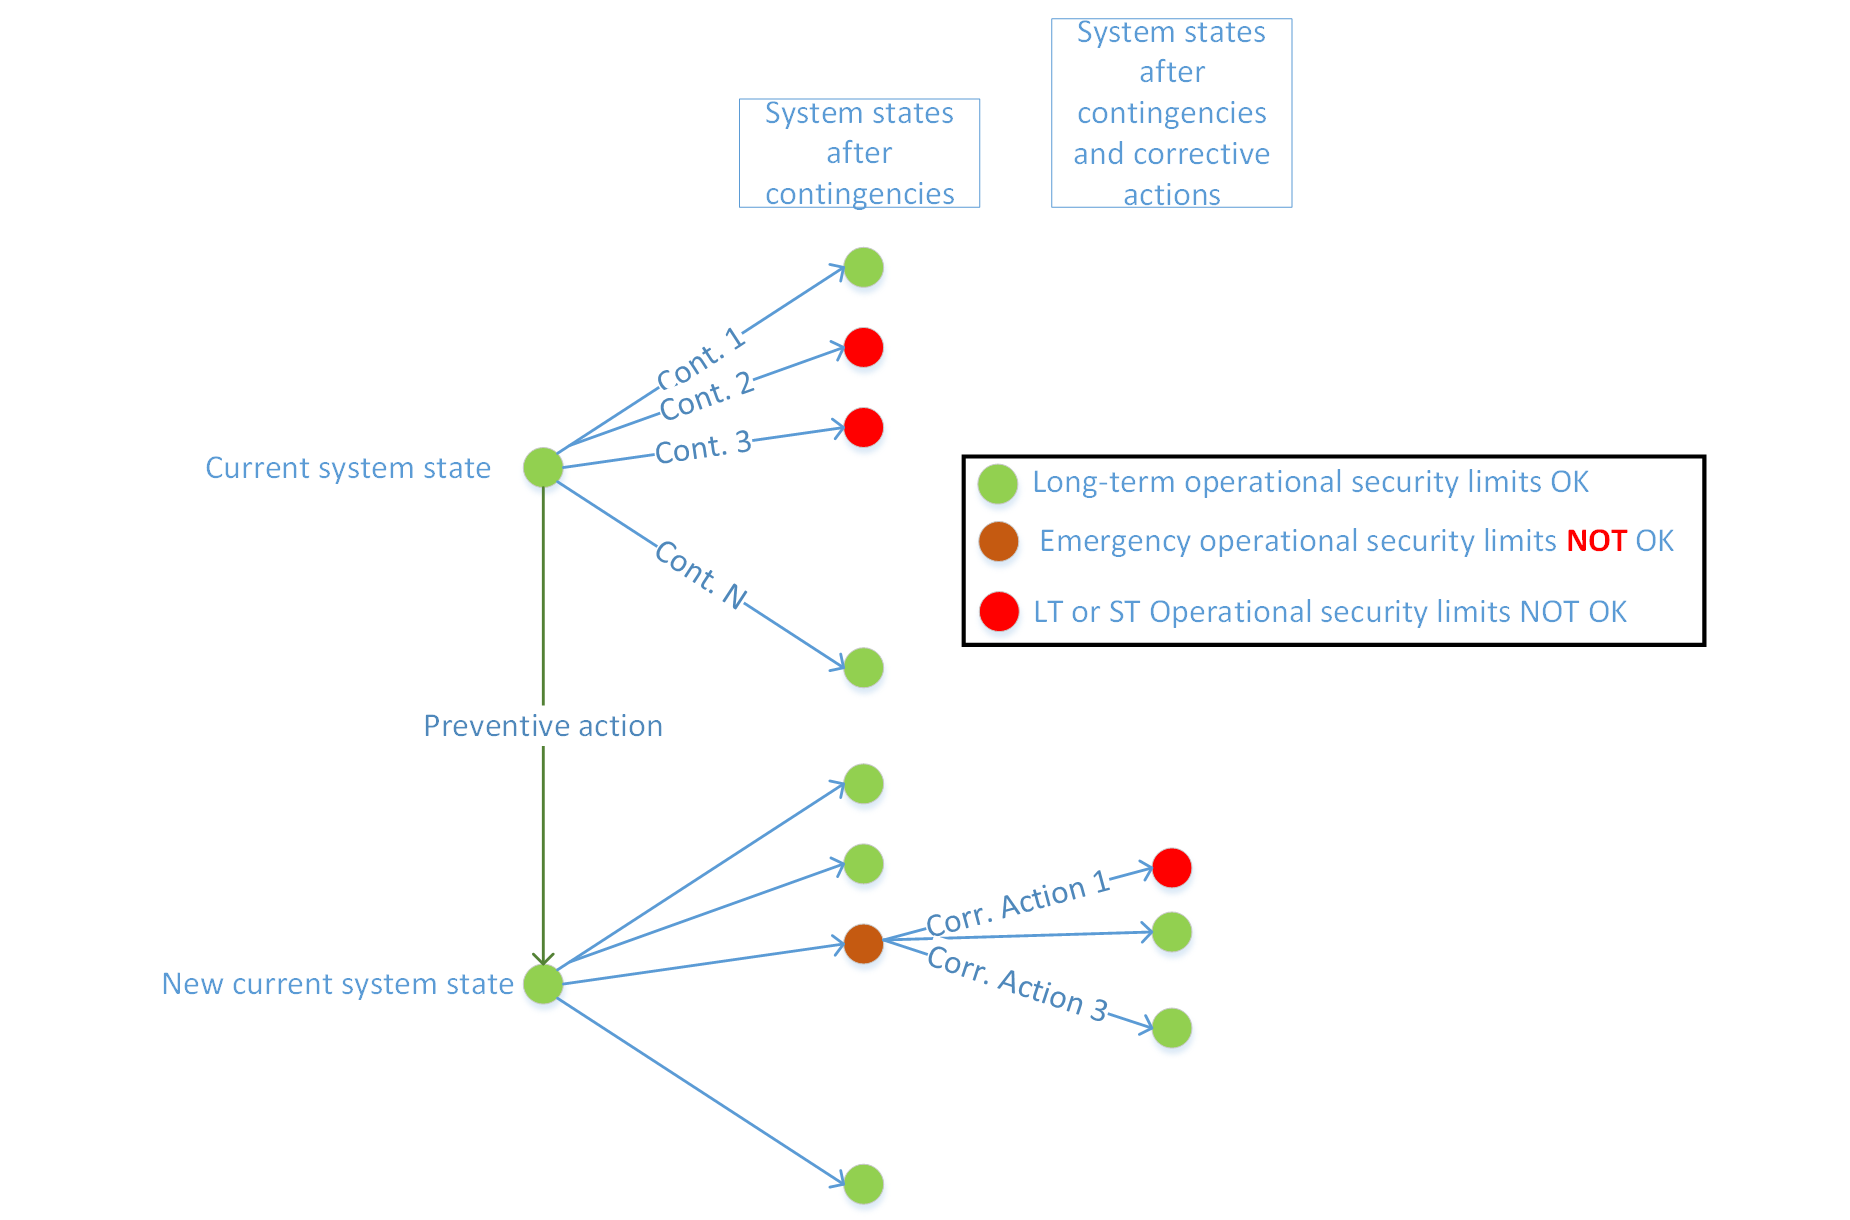
\includegraphics[width=1\textwidth]{Figs/Event-tree-prev-corr-actions-stlt-limits-wrong.png}}
\end{frame}

\begin{frame}
  \frametitle{Questions}
  \begin{itemize}
  \item What do we mean by ``system state''? How to determine it?
  \item What is the difference between OPF and SCOPF?
  \item Two examples of situations in which TSOs can make use of SCOPF.
  \end{itemize}
\end{frame}

\section{Solving SCOPF}


\begin{frame}
  \frametitle{Challenges}
  \begin{itemize}
  \item SCOPFs are nonlinear nonconvex optimization problems.
  \item Needless to say, there are challenging to solve.
  \item Challenge 1: Size of the problem (number of constraints and number of variables)
  \item Challenge 2: Nature of the problem for the full AC formulation (nonlinear nonconvex) $\Rightarrow$ Solving such problems is hard.
  \item Challenge 3: Including all possible types of control (including discrete control actions such as tap changer actions and line switching) $\Rightarrow$ Mixed integer optimization problem $\Rightarrow$ Even harder problem!
  \end{itemize}
\end{frame}

\begin{frame}
  \frametitle{State-of-the-art}
Read these three excellent sources:
\begin{itemize}
\item Capitanescu, ``Critical review of recent advances and further developments needed in AC optimal power flow,'' 2016.
\item Stott and Alsaç, ``Optimal power flow–basic requirements for real-life problems and their solutions,'' 2012.
\item FERC, ``Optimal power flow and formulation papers'', \url{https://www.ferc.gov/industries/electric/indus-act/market-planning/opf-papers.asp}
\end{itemize}
\end{frame}

\begin{frame}
  \frametitle{Solution method}
General solution method:\\
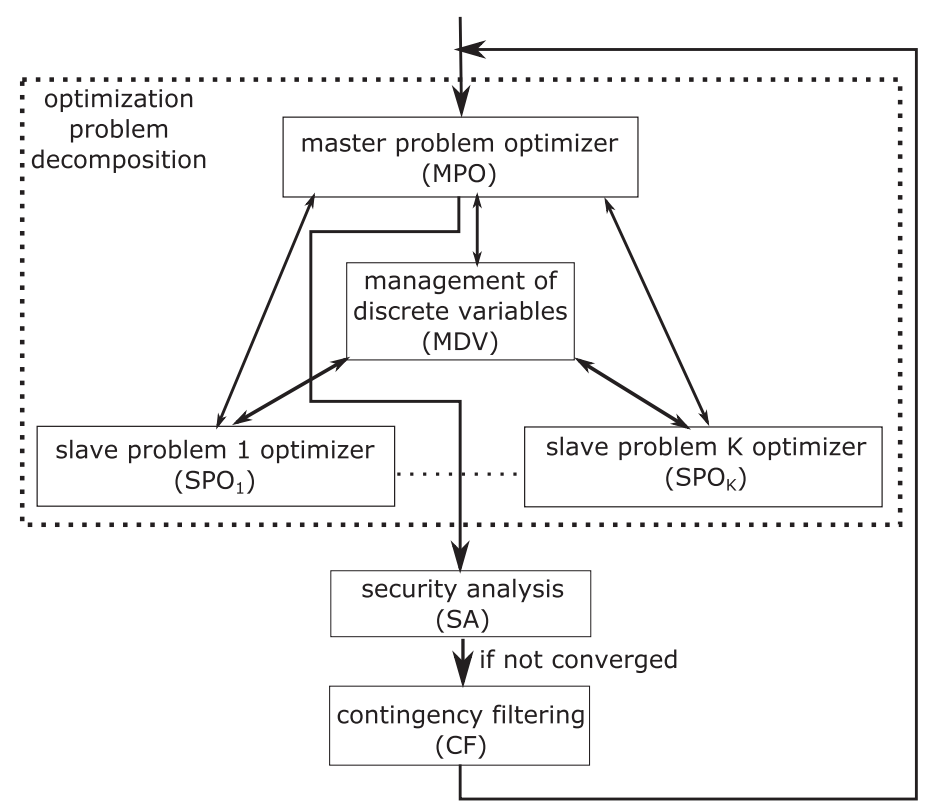
\includegraphics[width=0.7\textwidth]{Figs/SCOPF_flowchart.png}\\
From Capitanescu, ``Critical review of recent advances and further developments needed in AC optimal power flow,'' 2016.
\end{frame}

\begin{frame}
  \frametitle{In use today}
  \begin{itemize}
  \item DC-SCOPF implemented today by many independent system operators in the US for clearing the market.
  \item Some European TSOs have an implementation of an AC-SCOPF for real-time security optimization (every 15 minutes) (see for example López, 2015, ``Swiss TSO experience with an ac security-constrained optimal power flow application for real-time security management'').
  \end{itemize}
\end{frame}

\section{Conclusion}

\begin{frame}
  \frametitle{Take-home messages 1}
  \begin{itemize}
  \item Security = making sure that the system fulfils operational security limits even after contingencies occur.
  \item Contingency list to be considered = at least the N-1 contingencies.
  \item Preventive actions affect the system now and after any contingency occurs.
  \item Corrective actions affect the system only after a contingency occurs.
  \end{itemize}
\end{frame}

\begin{frame}
  \frametitle{Take-home messages 2}
  \begin{itemize}
  \item SCOPF is one tool to find preventive actions to apply now.
  \item Corrective actions are included in SCOPF to avoid being too conservative when finding preventive actions.
  \item Corrective actions determined by SCOPF can of course be used should contingencies actually occur.
  \item Preventive versus Preventive-Corrective versus Improved Preventive-Corrective SCOPF.
  \item AC SCOPF is a hard problem to solve.
  \item SCOPF is a mathematical tool for solving a power system problem. Don't lose the underlying power system problem (when does it arise? why do we want to use SCOPF? What are the physical phenomena involved? \ldots)!
  \end{itemize}
\end{frame}

%\section{References}
\begin{frame}[allowframebreaks]
\frametitle{References}
\printbibliography
\end{frame}

\end{document}
%%% Local Variables:
%%% mode: latex
%%% TeX-master: t
%%% End:
